\documentclass[aspectratio=169, 11pt]{beamer}

% --- PACKAGES ---
\usepackage[utf8]{inputenc}
\usepackage[T1]{fontenc}
\usepackage[french]{babel}
\usepackage{graphicx}
\usepackage{booktabs}
\usepackage{amsmath}
\usepackage{tikz}
\usetikzlibrary{arrows.meta, positioning}

% --- THÈME ---
\usetheme{Madrid}
\usecolortheme{whale}

\definecolor{dota_dark}{RGB}{18, 18, 36}
\definecolor{dota_accent}{RGB}{233, 69, 96}
\definecolor{dota_blue}{RGB}{52, 152, 219}
\definecolor{dota_green}{RGB}{46, 204, 113}
\definecolor{dota_gold}{RGB}{241, 196, 15}

\setbeamercolor{palette primary}{bg=dota_dark, fg=white}
\setbeamercolor{palette secondary}{bg=dota_dark!80, fg=white}
\setbeamercolor{palette tertiary}{bg=dota_accent, fg=white}
\setbeamercolor{structure}{fg=dota_accent}
\setbeamercolor{title}{fg=white, bg=dota_dark}
\setbeamercolor{frametitle}{fg=white, bg=dota_dark}
\setbeamercolor{block title}{bg=dota_accent, fg=white}
\setbeamercolor{block body}{bg=dota_dark!10}
\setbeamercolor{item}{fg=dota_accent}

\setbeamerfont{title}{size=\LARGE, series=\bfseries}
\setbeamerfont{frametitle}{size=\large, series=\bfseries}

\setbeamertemplate{footline}{
  \leavevmode\hbox{%
    \begin{beamercolorbox}[wd=.33\paperwidth,ht=2.5ex,dp=1ex,left]{palette primary}
      \hspace*{2ex}\insertshortauthor
    \end{beamercolorbox}%
    \begin{beamercolorbox}[wd=.34\paperwidth,ht=2.5ex,dp=1ex,center]{palette secondary}
      \insertshorttitle
    \end{beamercolorbox}%
    \begin{beamercolorbox}[wd=.33\paperwidth,ht=2.5ex,dp=1ex,right]{palette primary}
      \insertframenumber{} / \inserttotalframenumber\hspace*{2ex}
    \end{beamercolorbox}%
  }
}
\setbeamertemplate{navigation symbols}{}

% --- MÉTADONNÉES ---
\title{Dota 2 Trajectory Analyzer}
\subtitle{Compression MDL de trajectoires spatio-temporelles}
\author{Elias \textsc{Okat} \and Uzay \textsc{Turkmenel} \and Paul \textsc{Aubert}}
\institute{Université de Caen Normandie — L3 Informatique}
\date{Projet 2 — 2025-2026}

\begin{document}

% ============================================================================
\begin{frame}[plain]
\titlepage
\end{frame}

% ============================================================================
% PARTIE 1 — INTRODUCTION (2-3 slides)
% ============================================================================
\section{Introduction}

% --- SLIDE 1 : Contexte ---
\begin{frame}{Contexte : DotA 2 et les données}

\begin{columns}[c]
\begin{column}{0.45\textwidth}
    \textbf{DotA 2} — MOBA compétitif, 2$\times$5 joueurs

    \vspace{0.2cm}
    Chaque match $\approx$ 30-45 min $\Rightarrow$ \textbf{flux massif} de $(X,Y)$

    \vspace{0.2cm}
    \textbf{Trois obstacles majeurs :}
    \begin{enumerate}
        \item \textcolor{dota_accent}{\textbf{Données}} — +10M
        \item \textcolor{dota_accent}{\textbf{Bruit}} — micro-déplacements
        \item \textcolor{dota_accent}{\textbf{Calculs et exploitation}} — coûteux, interprétation complexe
    \end{enumerate}

    \vspace{0.2cm}
    \begin{block}{Question}
    Comment trier et exploiter ces données ? 
    \end{block}
\end{column}
\begin{column}{0.52\textwidth}
    \centering
    \makebox[\linewidth][c]{
        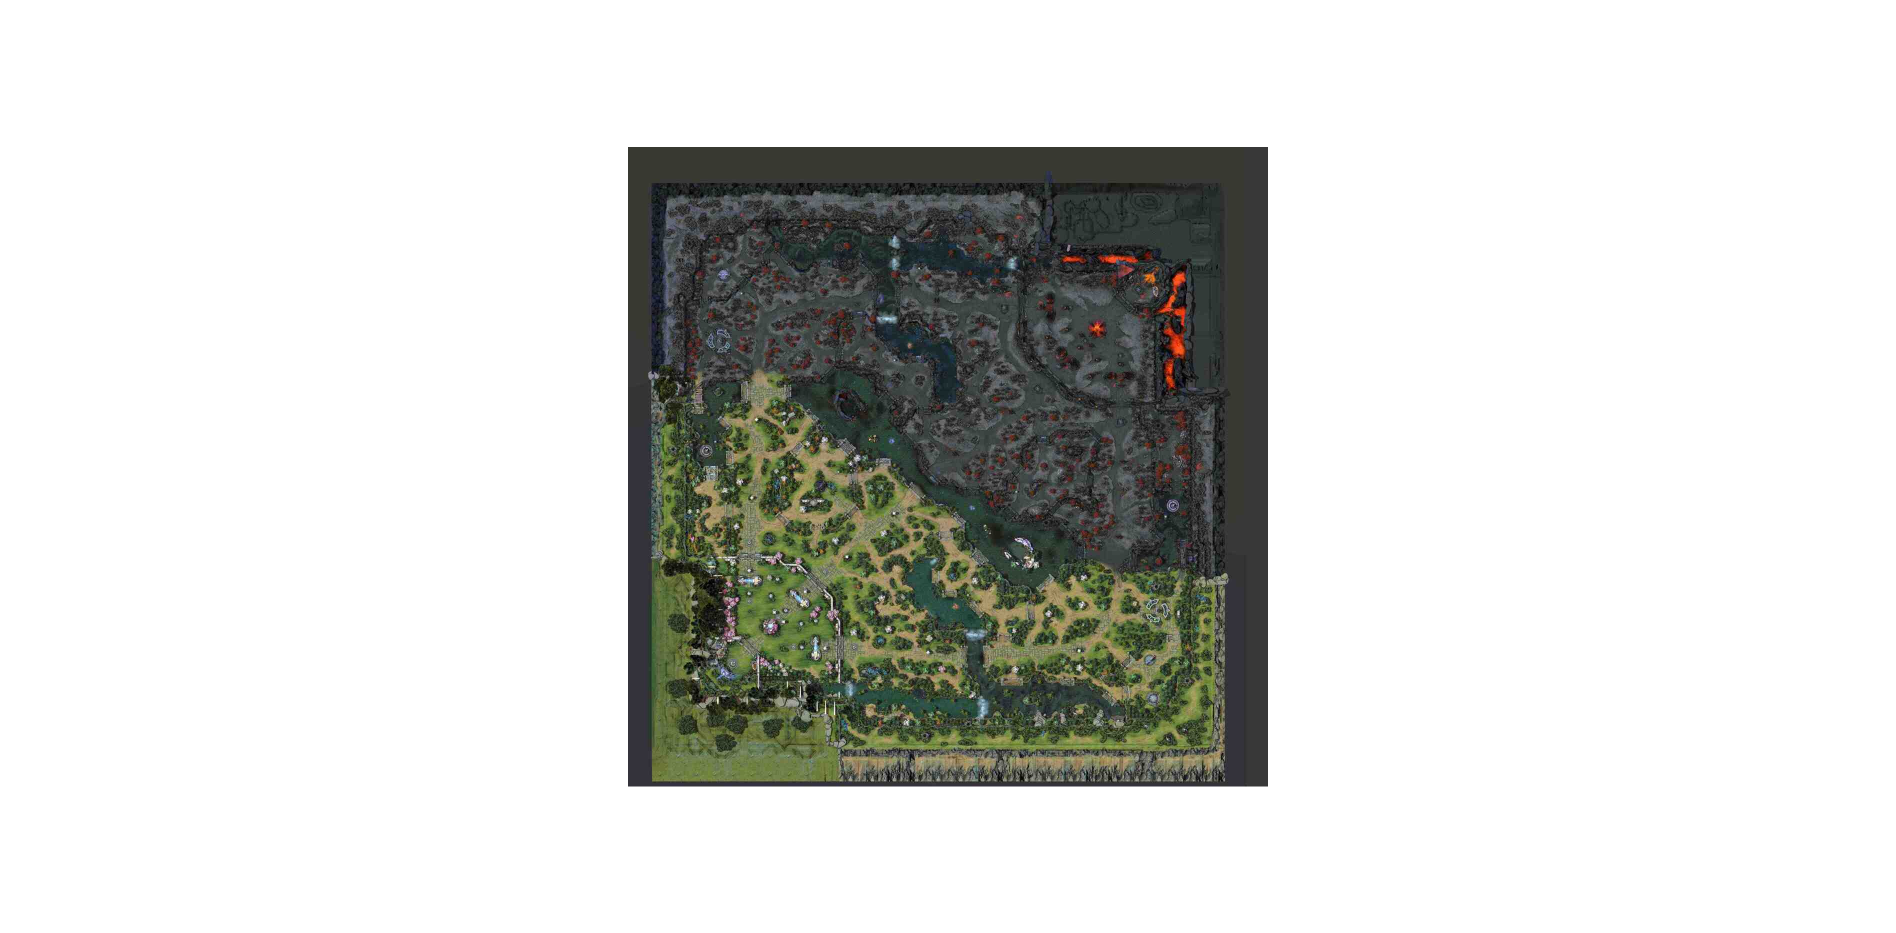
\includegraphics[width=1.9\linewidth]{img/canvas.png}
    }\\ % Fin de la ligne
    \vspace{-0.8cm} % Remonte le texte de 0.8 cm (ajuste la valeur si besoin)
    {\scriptsize Carte officielle de DotA 2}
\end{column}
\end{columns}

\end{frame}

% --- SLIDE 2 : Limites de l'état de l'art ---
\begin{frame}{Pourquoi les approches existantes ne suffisent pas}

\begin{columns}[T]
\begin{column}{0.48\textwidth}
    \textbf{1. Heatmaps statiques}
    \begin{itemize}
        \item Montrent \textit{où} les joueurs vont\ldots
        \item \textcolor{dota_accent}{Écrasent le temps} : pas de séquence
        \item Jungle $\to$ Mid $\to$ Rivière\ ? Invisible.
    \end{itemize}

    \vspace{0.3cm}
    \textbf{2. Grilles manuelles}
    \begin{itemize}
        \item Découpage arbitraire de la carte
        \item \textcolor{dota_accent}{Biais humain} aux frontières
        \item Ne s'adapte pas aux flux réels
    \end{itemize}
\end{column}
\begin{column}{0.48\textwidth}
    \textbf{3. Clustering direct sur points bruts}
    \begin{itemize}
        \item Matrice $N \times N$ : $N = 10$M $\Rightarrow$ \textcolor{dota_accent}{\textbf{impossible}}
        \item Le bruit noie le signal
    \end{itemize}

    \vspace{0.4cm}
    \begin{alertblock}{Constat}
    Il faut d'abord \textbf{comprimer} les données pour rendre toute analyse possible.
    \end{alertblock}

    \vspace{0.2cm}
    $\Rightarrow$ Notre approche : un pipeline en \textbf{3 phases}
\end{column}
\end{columns}

\end{frame}

% --- SLIDE 3 : Pipeline global ---
\begin{frame}{Notre pipeline en 3 phases}

\centering
\vspace{0.3cm}

\begin{columns}[c]
\begin{column}{0.01\textwidth}\end{column}
\begin{column}{0.27\textwidth}
    \centering
    {\footnotesize\textcolor{dota_blue}{10M points}}\\[0.15cm]
    \colorbox{dota_blue}{\parbox{0.9\linewidth}{\centering\color{white}\textbf{Phase 1}\\[0.1cm]Compression\\MDL}}
\end{column}
\begin{column}{0.06\textwidth}
    \centering
    {\Large\textcolor{gray}{$\Longrightarrow$}}\\
    {\tiny\textcolor{gray}{segments}}
\end{column}
\begin{column}{0.27\textwidth}
    \centering
    {\footnotesize\textcolor{dota_accent}{18\,000 segments}}\\[0.15cm]
    \colorbox{dota_accent}{\parbox{0.9\linewidth}{\centering\color{white}\textbf{Phase 2}\\[0.1cm]Clustering\\TRACLUS + AP}}
\end{column}
\begin{column}{0.06\textwidth}
    \centering
    {\Large\textcolor{gray}{$\Longrightarrow$}}\\
    {\tiny\textcolor{gray}{zones}}
\end{column}
\begin{column}{0.27\textwidth}
    \centering
    {\footnotesize\textcolor{dota_green!70!black}{10 macro-zones}}\\[0.15cm]
    \colorbox{dota_green!70!black}{\parbox{0.9\linewidth}{\centering\color{white}\textbf{Phase 3}\\[0.1cm]Fouille de motifs\\PrefixSpan}}
\end{column}
\begin{column}{0.01\textwidth}\end{column}
\end{columns}

\vspace{0.6cm}

\begin{columns}[T]
\begin{column}{0.32\textwidth}
    \centering
    \textcolor{dota_blue}{\textbf{Réduire}}\\
    {\small Compression MDL :\\
    $-$96\% de volume\\
    Bruit filtré}
\end{column}
\begin{column}{0.32\textwidth}
    \centering
    \textcolor{dota_accent}{\textbf{Structurer}}\\
    {\small Distance TRACLUS\\
    Affinity Propagation\\
    $\to$ 10 zones automatiques}
\end{column}
\begin{column}{0.32\textwidth}
    \centering
    \textcolor{dota_green!70!black}{\textbf{Interpréter}}\\
    {\small PrefixSpan :\\
    Motifs séquentiels\\
    $=$ stratégies de jeu}
\end{column}
\end{columns}

\end{frame}

% --- SLIDE : Diagramme de classes ---
\begin{frame}{Architecture logicielle — Diagramme de classes}
\centering
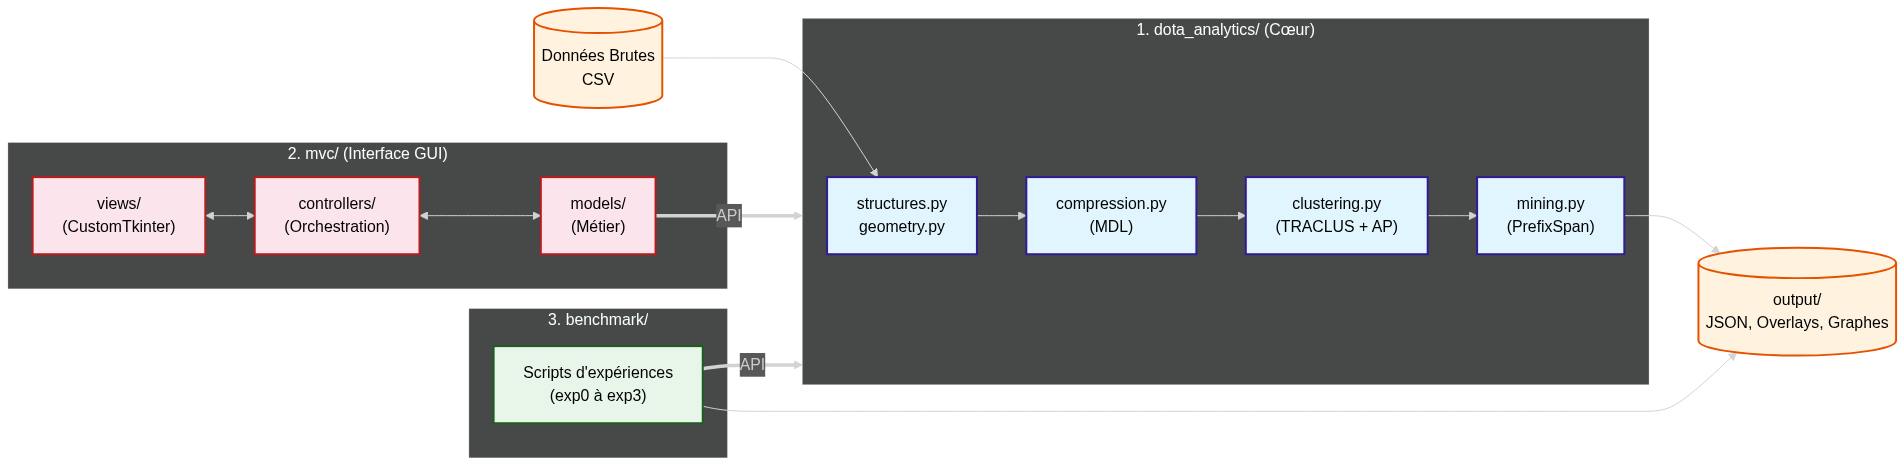
\includegraphics[width=\textwidth, height=0.88\textheight, keepaspectratio]{img/diagramme_architech.jpg}
\end{frame}

% --- SLIDE : Choix du langage ---
\begin{frame}{Choix technologique : Python scientifique}
\small
\begin{columns}[T]
\begin{column}{0.48\textwidth}

    \textbf{Pourquoi Python ?}
    \begin{itemize}\setlength{\itemsep}{1pt}
        \item Écosystème \textbf{data science} mature
        \item Prototypage rapide, code lisible
        \item Interopérabilité C/Fortran via NumPy
    \end{itemize}

    \vspace{0.15cm}
    \textbf{NumPy} — calcul matriciel
    \begin{itemize}\setlength{\itemsep}{1pt}
        \item Matrices de distance $N \times N$ (TRACLUS)
        \item Vectorisation : \textcolor{dota_green}{\textbf{$\times$100}} vs boucles Python
        \item Mémoire efficace (\texttt{float32})
    \end{itemize}

\end{column}
\begin{column}{0.48\textwidth}

    \textbf{Matplotlib} — visualisation
    \begin{itemize}\setlength{\itemsep}{1pt}
        \item Superposition trajectoires sur carte
        \item Graphiques multi-panneaux (benchmarks)
    \end{itemize}

    \vspace{0.15cm}
    \textbf{Autres dépendances :}
    \begin{itemize}\setlength{\itemsep}{1pt}
        \item \texttt{scikit-learn} — Silhouette, Davies-Bouldin
        \item \texttt{scipy} — Hausdorff, distances spatiales
    \end{itemize}

    

\end{column}
\end{columns}

\end{frame}

% ============================================================================
% PARTIE 2 — MDL
% ============================================================================
\section{Compression MDL}

% --- SLIDE 4a : Principe MDL ---
\begin{frame}{MDL — Principe et algorithme glouton}

\begin{columns}[T]
\begin{column}{0.48\textwidth}

\begin{block}{Idée clé (Minimum Description Length)}
La \textbf{description la plus courte} qui reste \textbf{fidèle} à la trajectoire (erreur $< w_{error}$).
\end{block}

\vspace{0.2cm}

\textbf{Algorithme glouton :}
\begin{enumerate}\setlength{\itemsep}{0pt}
    \item Partir du premier point
    \item \textbf{Étendre} le segment point par point
    \item Calculer $d_\perp$ de chaque intermédiaire
    \item $\max(d_\perp) < w_{error}$ $\Rightarrow$ continuer \textcolor{dota_green}{\checkmark}
    \item $\max(d_\perp) \geq w_{error}$ $\Rightarrow$ \textbf{couper} \textcolor{dota_accent}{\textbf{$\times$}}
    \item Reprendre au dernier point validé
\end{enumerate}

\end{column}
\begin{column}{0.48\textwidth}

    \textbf{$w_{error}$} = tolérance max :
    \begin{itemize}\setlength{\itemsep}{0pt}
        \item Petit $\to$ haute fidélité, peu de compression
        \item Grand $\to$ forte compression, perte de détail
        \item \textcolor{dota_accent}{\textbf{Notre choix : $w_{error} = 12$}}
    \end{itemize}

    \vspace{0.2cm}
    {\small Complexité : $\mathcal{O}(N^2)$ pire cas, $\sim\mathcal{O}(N^{1.5})$ en pratique}

    \vspace{0.2cm}
    \begin{alertblock}{Résultat}
    Compression \textbf{96--98\%} du volume, bruit filtré, erreur bornée.
    \end{alertblock}
\end{column}
\end{columns}

\end{frame}

% --- SLIDE 5 : Avant / après ---
\begin{frame}{Résultat : avant / après compression}

\begin{columns}[c]
\begin{column}{0.48\textwidth}
    \centering
    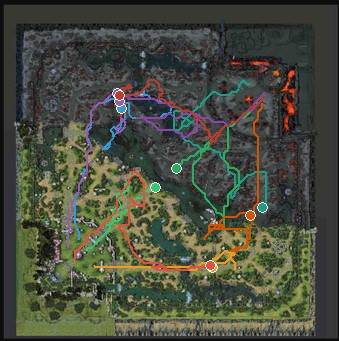
\includegraphics[width=0.9\linewidth]{img/brut.jpg}

    \vspace{0.1cm}
    \textbf{Trajectoire brute}\\
    {\scriptsize Milliers de points, bruit inclus}
\end{column}
\begin{column}{0.04\textwidth}
    \centering
    {\LARGE $\boldsymbol{\to}$}
\end{column}
\begin{column}{0.48\textwidth}
    \centering
    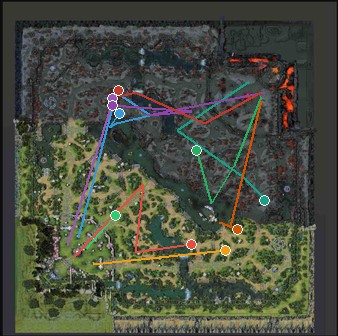
\includegraphics[width=0.9\linewidth]{img/compresser.jpg}

    \vspace{0.1cm}
    \textbf{Après MDL ($w_{error}=12$)}\\
    {\scriptsize $\sim$250 segments / joueur}
\end{column}
\end{columns}

\vspace{0.2cm}
\centering
{\small Compression \textcolor{dota_green}{\textbf{96--98\%}} — bruit supprimé, signal préservé, erreur max $< 12$ unités}

\end{frame}

% --- SLIDE : CSV brut vs JSON compressé ---
\begin{frame}{Données : du CSV brut au JSON compressé}

\begin{columns}[c]
\begin{column}{0.48\textwidth}
    \centering
    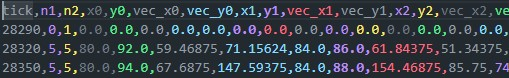
\includegraphics[width=\linewidth, height=0.72\textheight, keepaspectratio]{img/extrait_csv.jpg}

    \vspace{0.1cm}
    \textbf{Entrée — CSV brut}\\
    {\scriptsize $(x, y)$ toutes les 0{,}03\,s $\to$ milliers de lignes}
\end{column}
\begin{column}{0.04\textwidth}
    \centering
    {\LARGE $\boldsymbol{\to}$}
\end{column}
\begin{column}{0.48\textwidth}
    \centering
    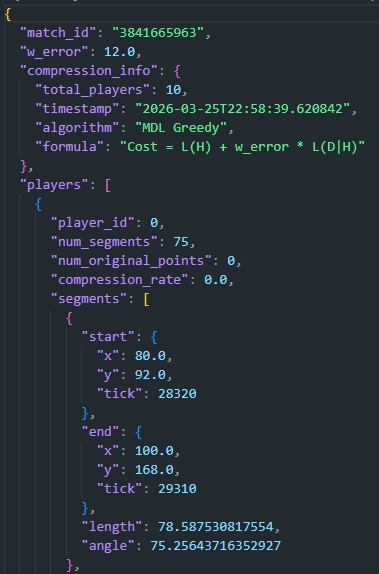
\includegraphics[width=\linewidth, height=0.72\textheight, keepaspectratio]{img/json_extrait.jpg}

    \vspace{0.1cm}
    \textbf{Sortie — JSON compressé}\\
    {\scriptsize Segments + labels de zones $\to$ exploitable par PrefixSpan}
\end{column}
\end{columns}

\centering
{\small Le pipeline transforme un flux brut de coordonnées en \textcolor{dota_green}{\textbf{séquences symboliques}} prêtes pour le \textit{mining}.}

\end{frame}

% ============================================================================
% PARTIE 3 — TRANSITION VERS LES EXPÉRIMENTATIONS
% ============================================================================
\section{Expérimentations}

% --- SLIDE : MDL vs Baselines ---
\begin{frame}{Exp. 1 — MDL \textit{vs} Uniforme \textit{vs} Douglas-Peucker}
\small
\begin{columns}[c]
\begin{column}{0.52\textwidth}
    \centering
    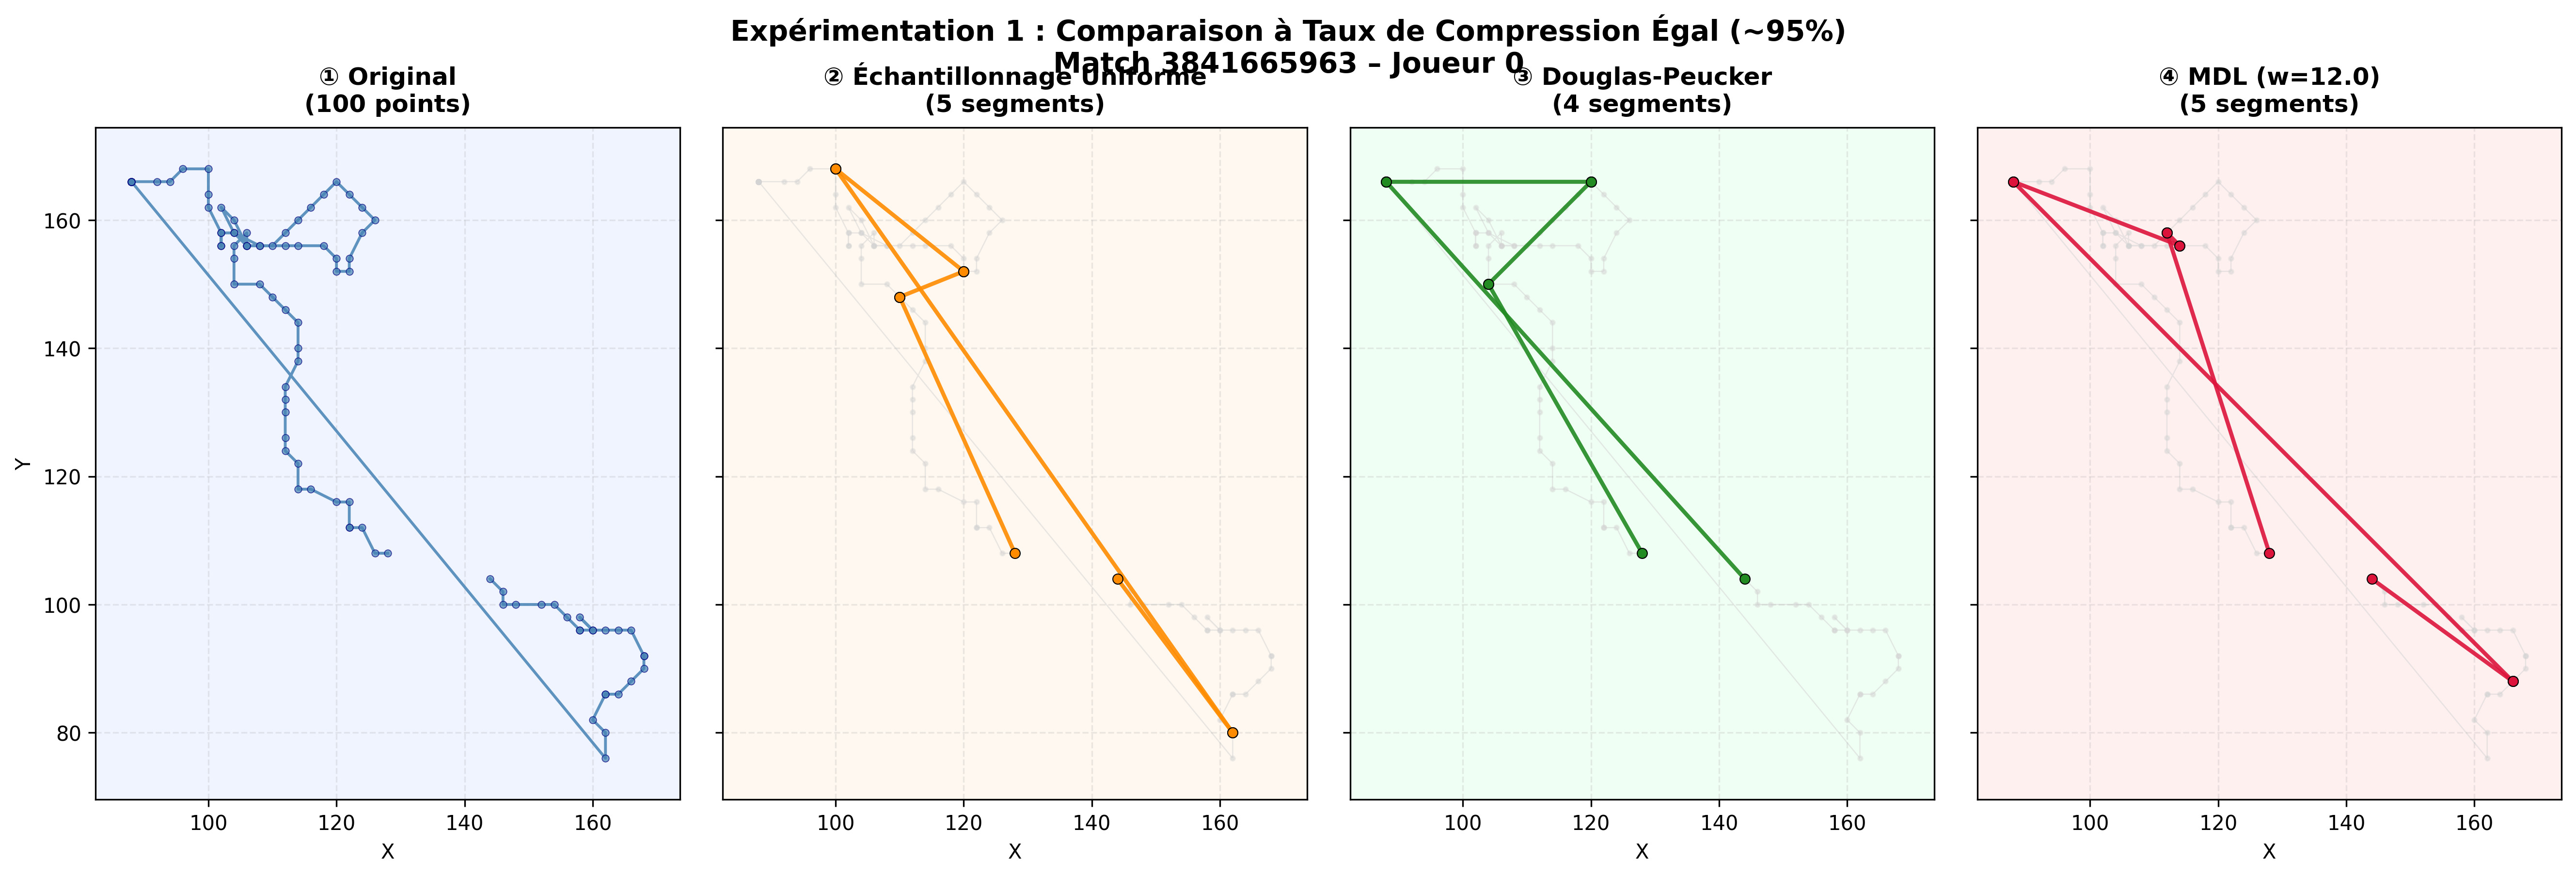
\includegraphics[width=\linewidth, height=0.7\textheight, keepaspectratio]{img/baseline_comparison.jpg}
\end{column}
\begin{column}{0.45\textwidth}
    À \textbf{compression égale} ($\sim$95\%) :

    \vspace{0.1cm}
    {\small\begin{tabular}{lcc}
    \toprule
    \textbf{Méthode} & \textbf{RMSE} & \textbf{Hausd.} \\
    \midrule
    Uniforme & 5.07 & 12.80 \\
    Douglas-P. & 10.81 & 22.09 \\
    \textcolor{dota_green}{\textbf{MDL}} & \textcolor{dota_green}{\textbf{5.48}} & \textcolor{dota_green}{\textbf{11.66}} \\
    \bottomrule
    \end{tabular}}

    \vspace{0.15cm}
    \begin{alertblock}{Verdict}
    {\small MDL : \textbf{meilleure fidélité} (Hausdorff min).}
    \end{alertblock}
\end{column}
\end{columns}
\end{frame}

% --- SLIDE : Complexité temporelle ---
\begin{frame}{Exp. 1b — Complexité temporelle : MDL \textit{vs} Baselines}
\small
\begin{columns}[c]
\begin{column}{0.52\textwidth}
    \centering
    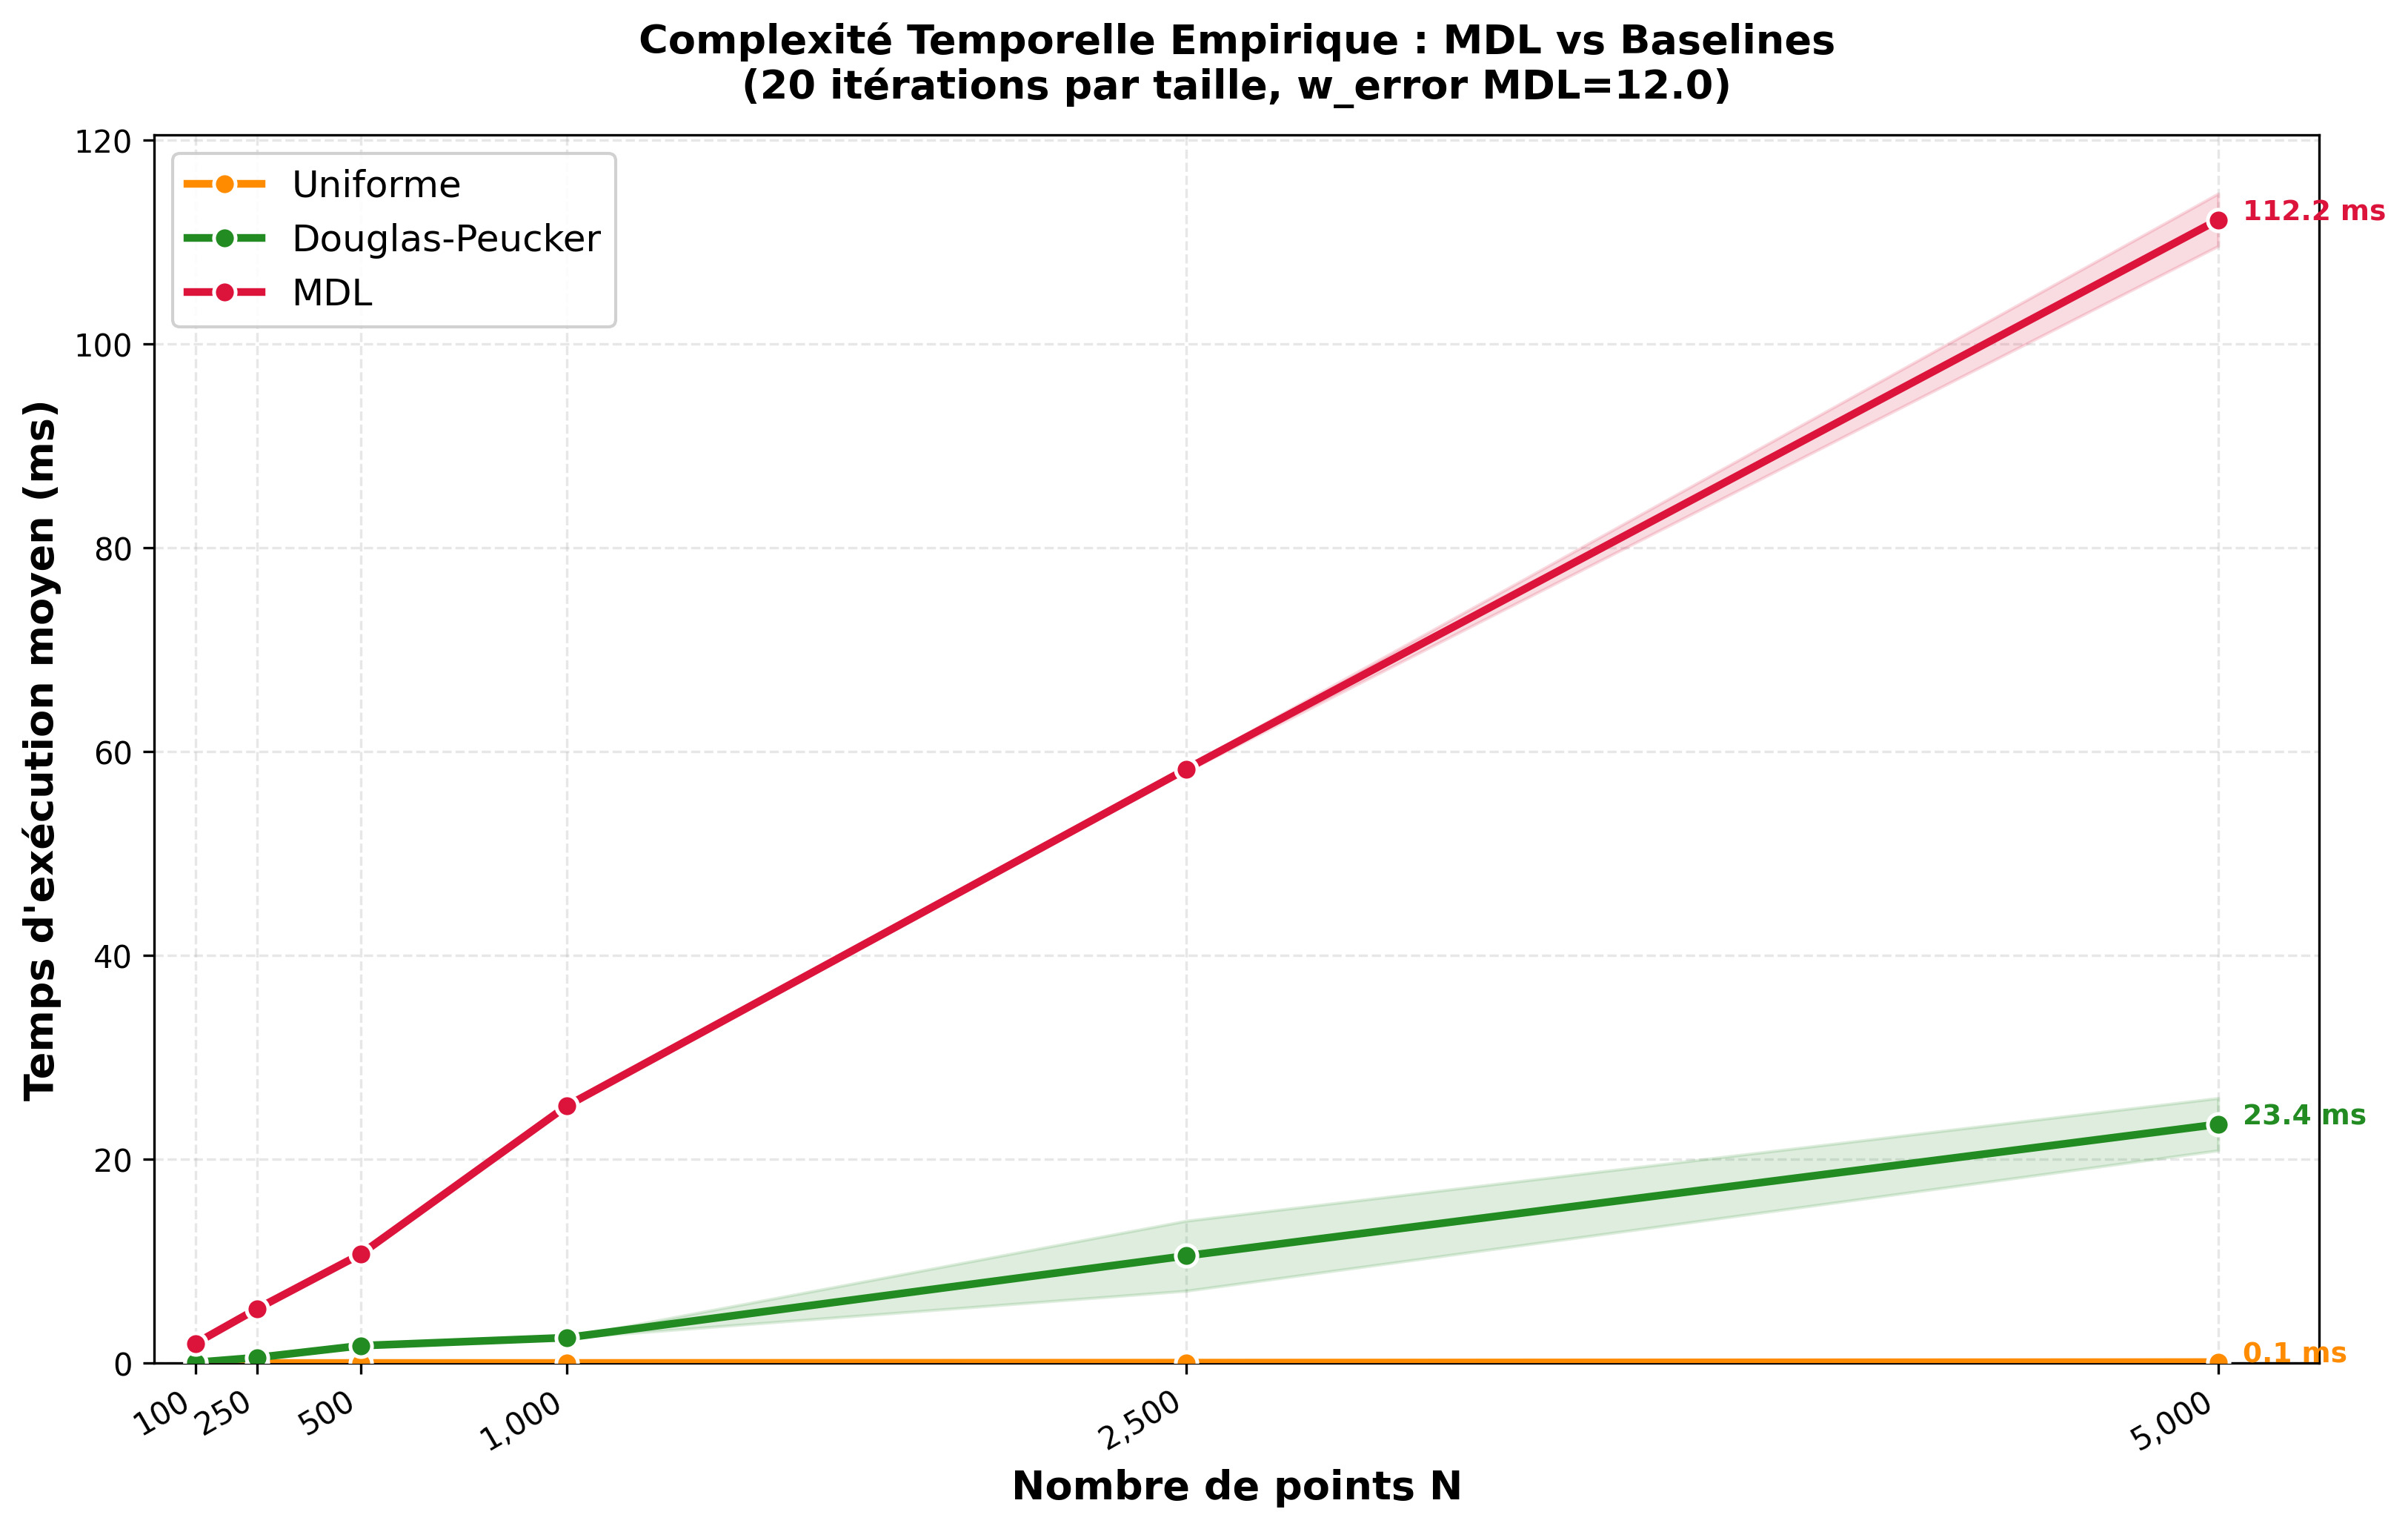
\includegraphics[width=\linewidth, height=0.7\textheight, keepaspectratio]{img/time_complexity_plot.jpg}
\end{column}
\begin{column}{0.45\textwidth}
    {\small\begin{tabular}{lcc}
    \toprule
    \textbf{Méthode} & \textbf{Complexité} & \textbf{5\,000 pts} \\
    \midrule
    Uniforme & $\mathcal{O}(1)$ & 0.1 ms \\
    Douglas-P. & $\mathcal{O}(N \log N)$ & 23 ms \\
    \textbf{MDL} & $\mathcal{O}(N^{1.5})$ & 112 ms \\
    \bottomrule
    \end{tabular}}

    \vspace{0.2cm}
    \begin{block}{Verdict}
    {\small MDL plus lent mais \textbf{acceptable} ($\sim$7s / match). Le coût se justifie par la \textbf{qualité}.}
    \end{block}
\end{column}
\end{columns}
\end{frame}

% --- SLIDE : Sensibilité w_error ---
\begin{frame}{Exp. 2 — Sensibilité de $w_{error}$ : pourquoi 12 ?}

\centering
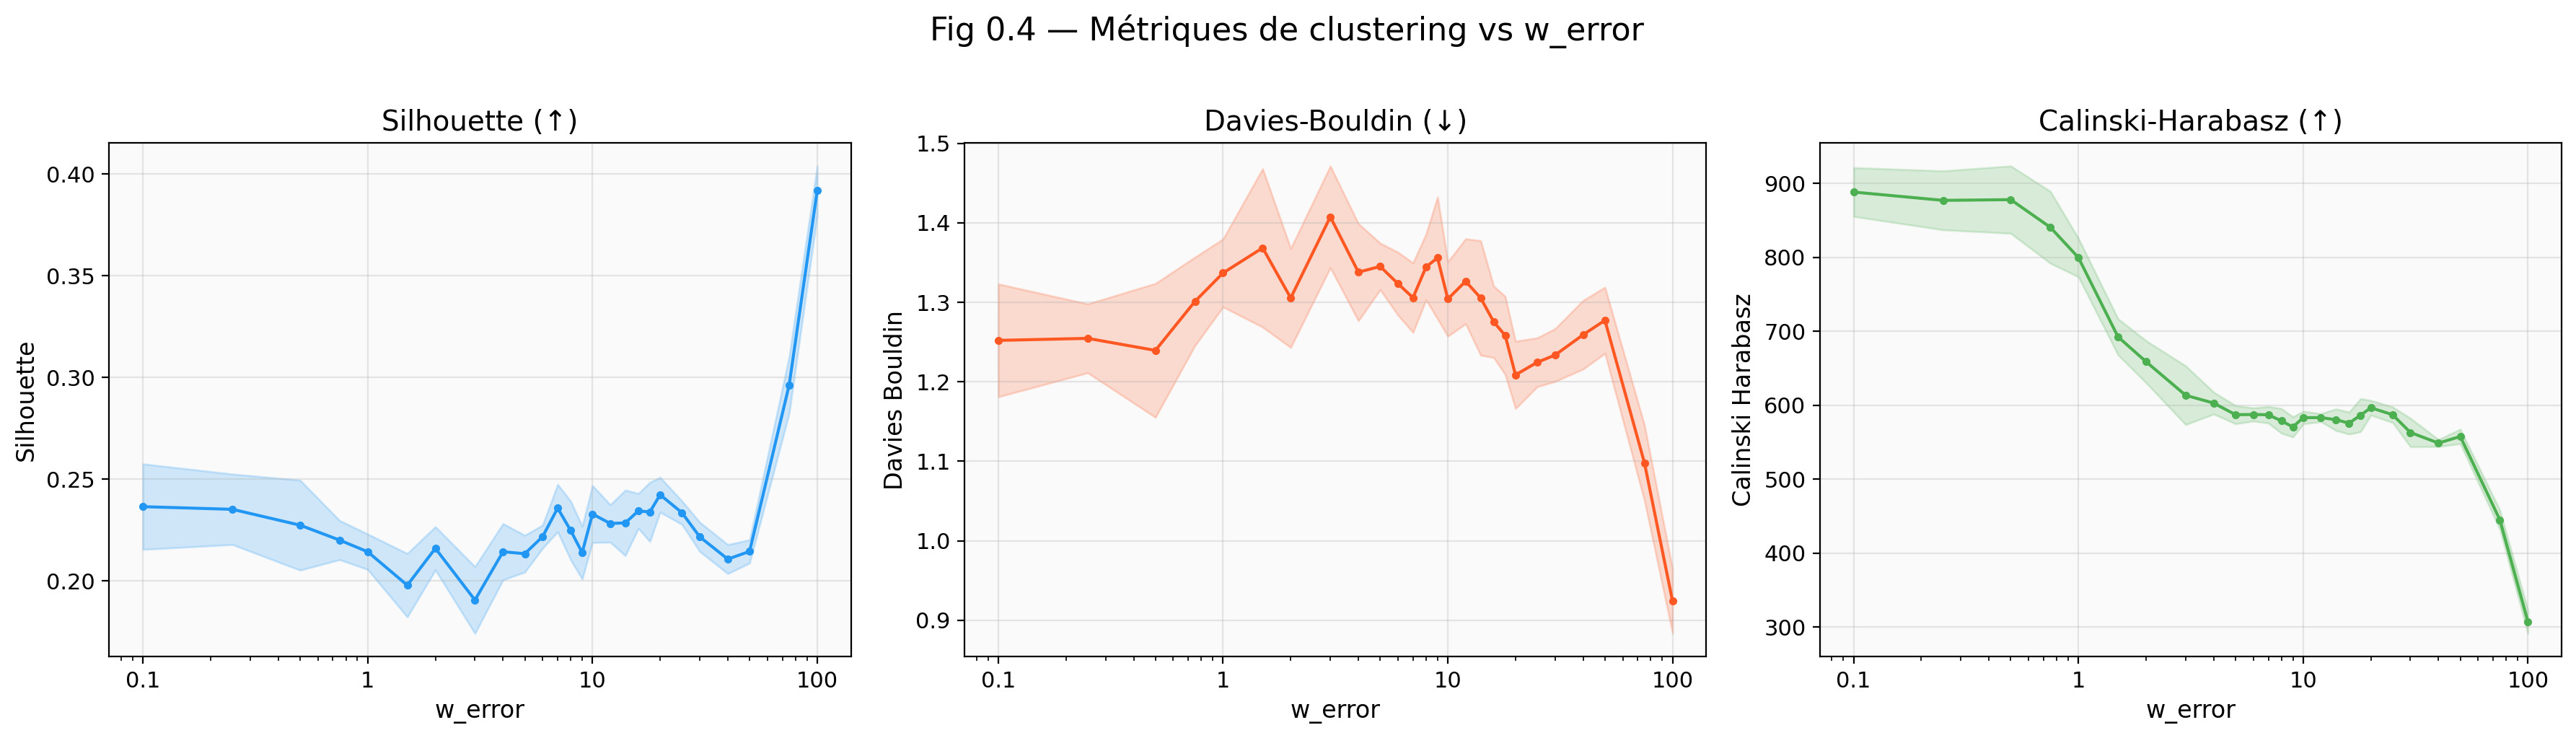
\includegraphics[width=0.70\linewidth]{img/fig0_4_panel_metrics_werror.jpg}

\vspace{0.15cm}

\begin{columns}[T]
\begin{column}{0.48\textwidth}
    \textbf{Observation :}
    \begin{itemize}
        \item $w_{error}$ petit $\to$ fidélité mais faible compression
        \item $w_{error}$ grand $\to$ plateau à $\sim$96\%
        \item \textbf{Coude} à $w_{error} \approx 12$
    \end{itemize}
\end{column}
\begin{column}{0.48\textwidth}
    \begin{block}{Conclusion}
    $w_{error} = 12$ = meilleur compromis compression / fidélité.\\
    Silhouette se stabilise, bruit $\sigma \leq 2$ absorbé.
    \end{block}
\end{column}
\end{columns}

\end{frame}

% --- SLIDE : Exp. 3 — Robustesse au bruit gaussien ---
\begin{frame}{Exp. 3 — Robustesse de MDL au bruit gaussien}

\centering
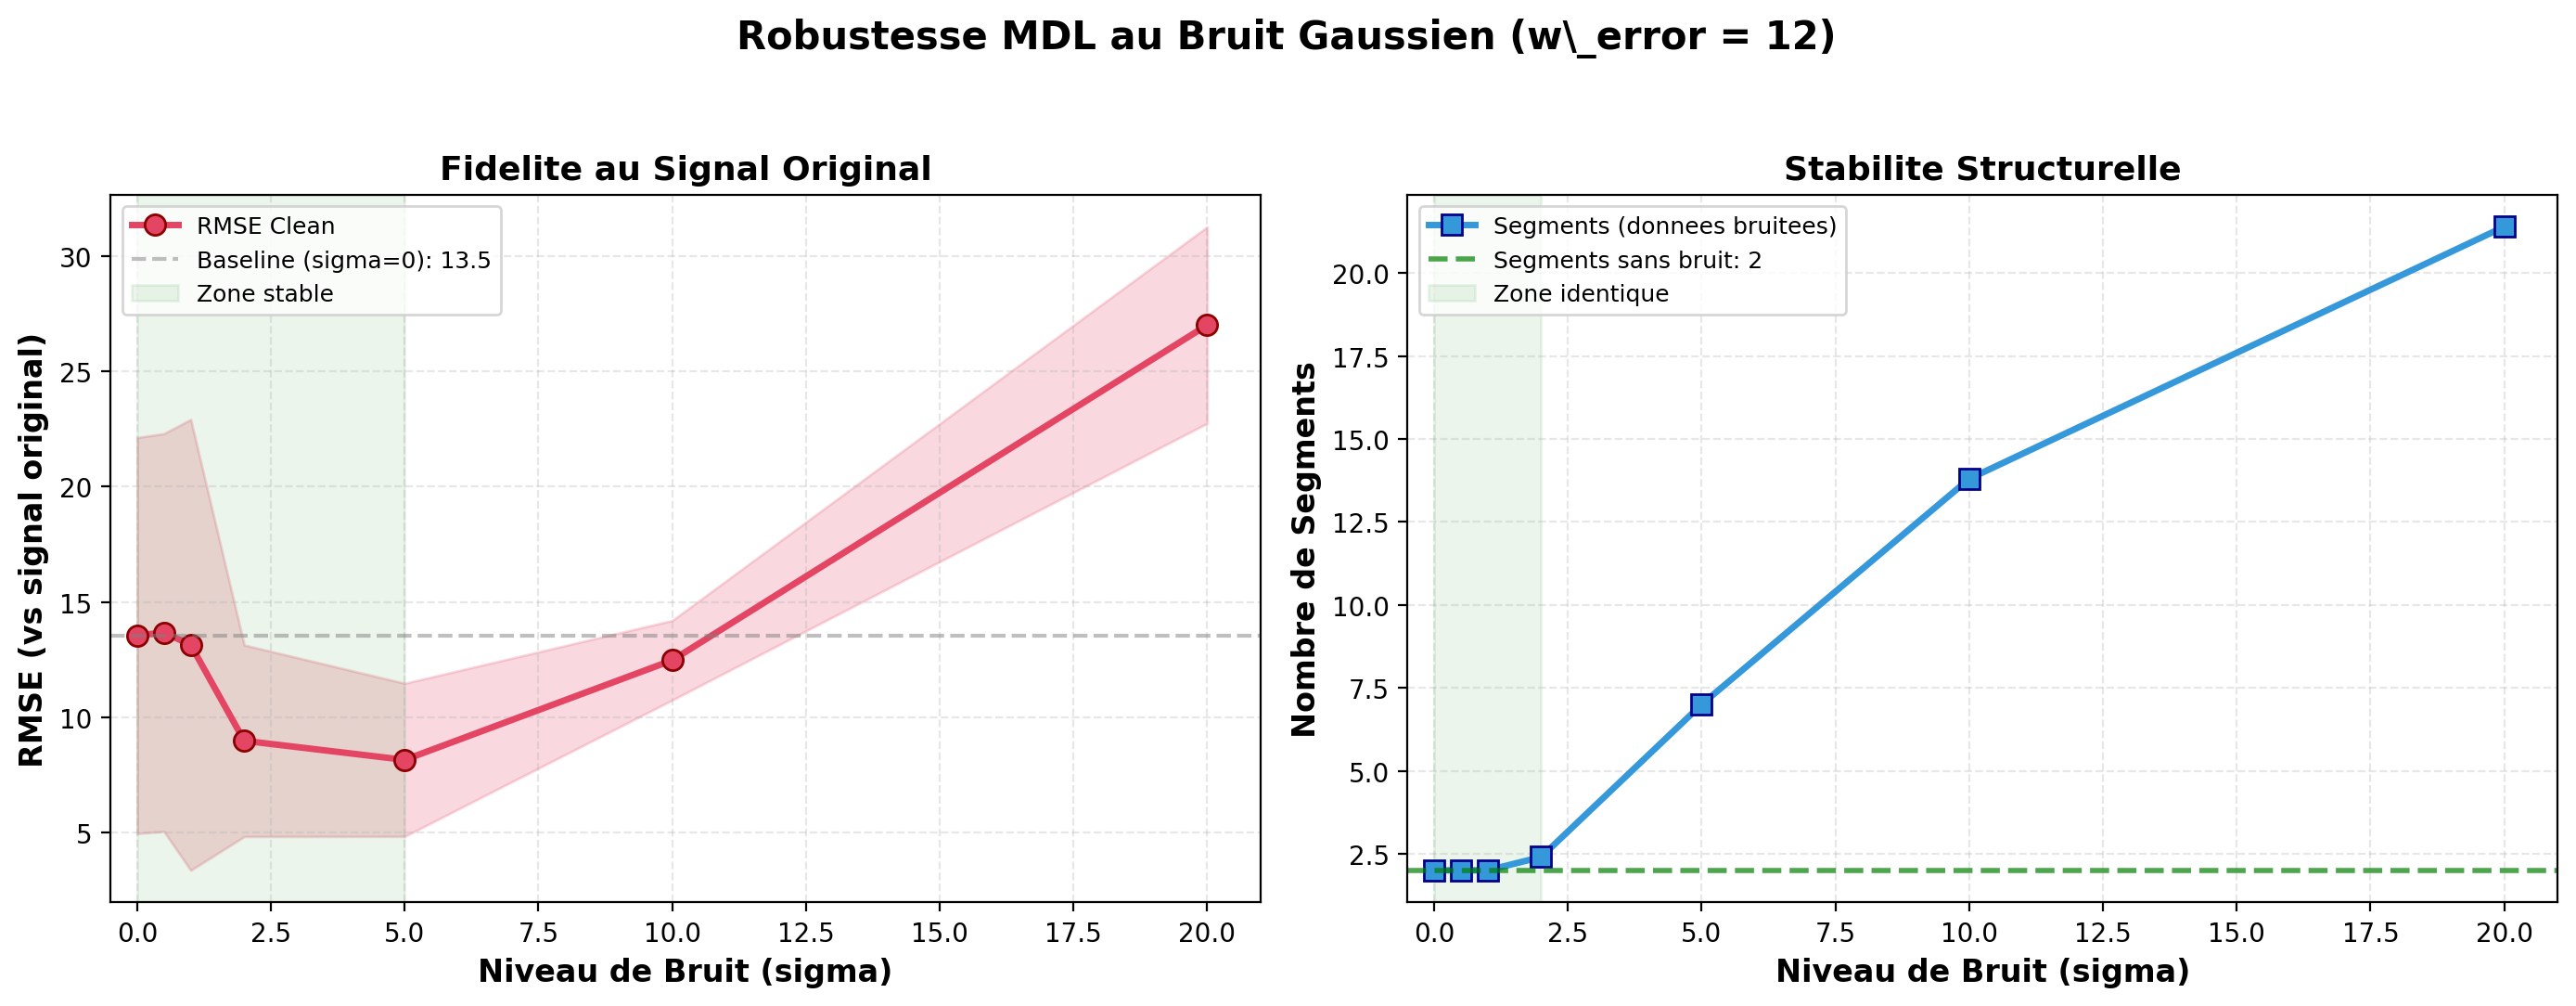
\includegraphics[width=0.75\linewidth]{img/robustesse_bruit_w12.png}

\vspace{0.1cm}

\begin{columns}[T]
\begin{column}{0.48\textwidth}
    {\small \textbf{Protocole :} injection de bruit $\mathcal{N}(0, \sigma^2)$ croissant sur 5 échantillons, compression MDL ($w_{error}=12$).}
\end{column}
\begin{column}{0.48\textwidth}
    \begin{block}{Résultat}
    {\small RMSE stable jusqu'à $\sigma=5$.\\
    Structure identique ($\sim$2 seg.) jusqu'à $\sigma=2$.\\
    MDL \textbf{filtre le bruit}, pas le signal.}
    \end{block}
\end{column}
\end{columns}

\end{frame}

% --- SLIDE : Triptyque robustesse visuelle ---
\begin{frame}{Exp. 3b — Visualisation : trajectoire propre $\to$ bruitée $\to$ filtrée}

\centering
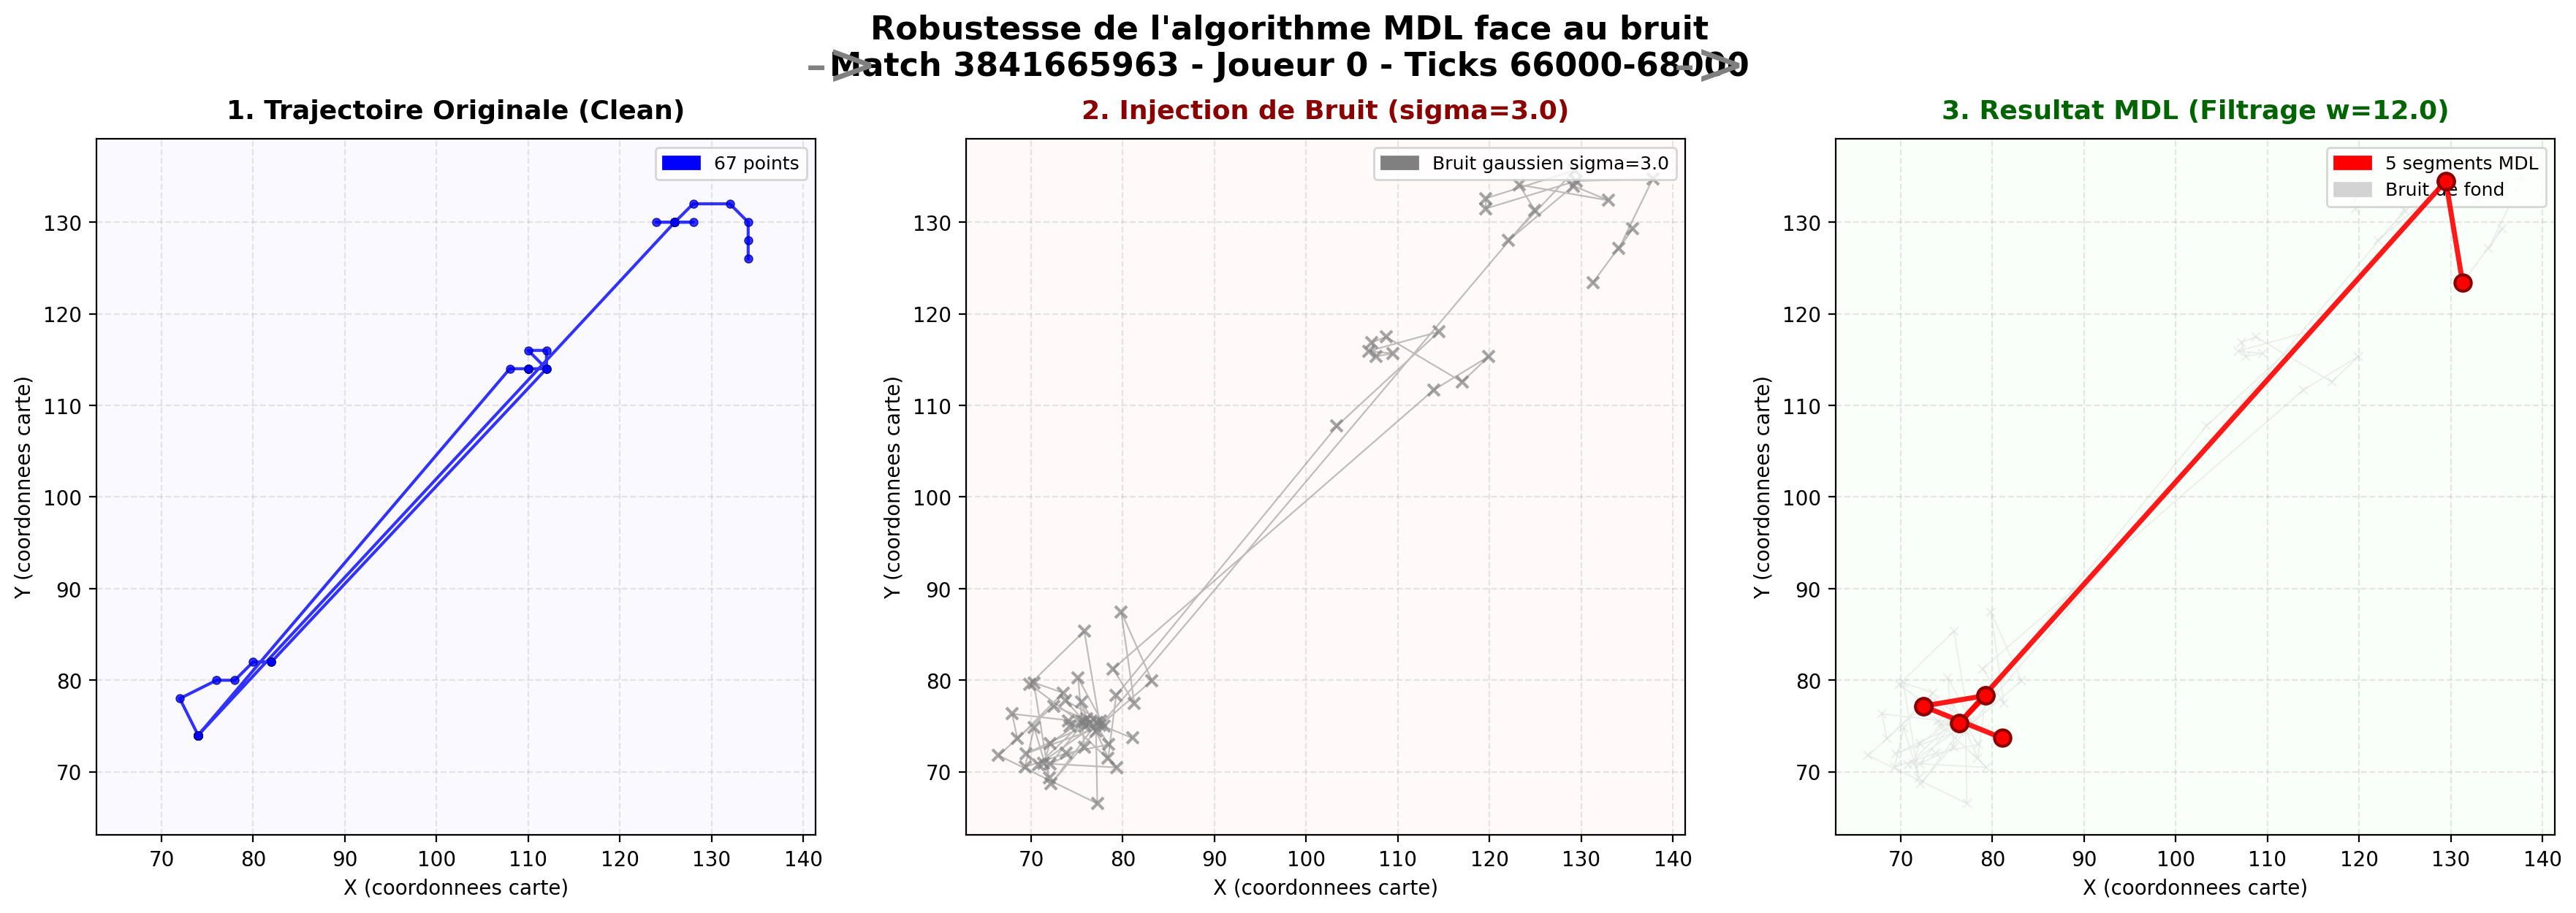
\includegraphics[width=0.95\linewidth, height=0.65\textheight, keepaspectratio]{img/triptych_w12_sigma3.jpg}

\vspace{0.2cm}

\begin{columns}[T]
\begin{column}{0.30\textwidth}
    \centering
    \textcolor{dota_blue}{\textbf{1. Originale}}\\
    {\small 67 points, trajectoire nette}
\end{column}
\begin{column}{0.30\textwidth}
    \centering
    \textcolor{gray}{\textbf{2. Bruit $\sigma=3$}}\\
    {\small Points dispersés, signal noyé}
\end{column}
\begin{column}{0.30\textwidth}
    \centering
    \textcolor{dota_accent}{\textbf{3. Après MDL}}\\
    {\small 5 segments, structure retrouvée}
\end{column}
\end{columns}

\vspace{0.15cm}
\centering
{\small MDL absorbe le bruit et \textcolor{dota_green}{\textbf{restitue la même structure}} que la trajectoire propre.}

\end{frame}

% --- SLIDE : Transition compression → clustering ---
\begin{frame}{Compression $\to$ Clustering : quel impact ?}
\small
\begin{columns}[c]
\begin{column}{0.55\textwidth}
    \centering
    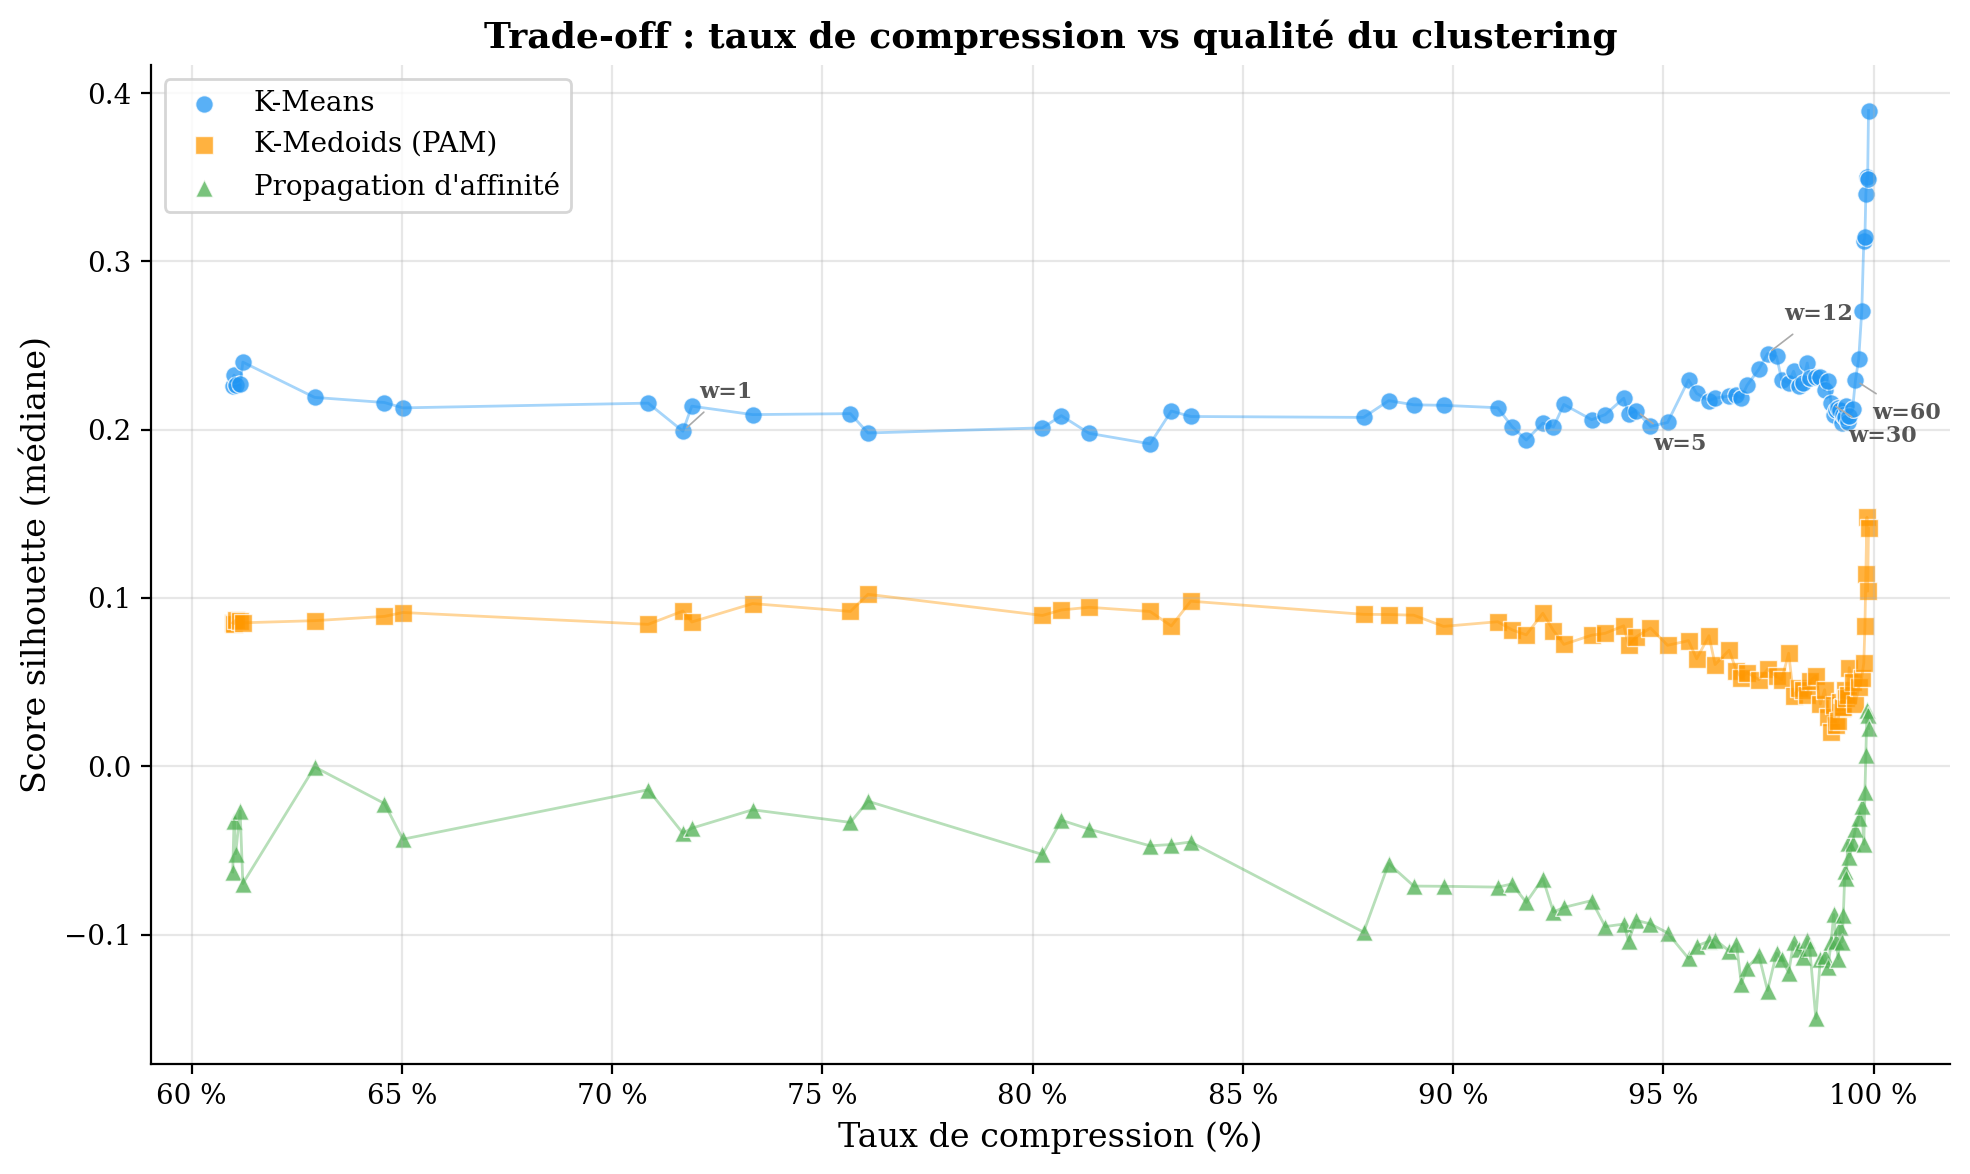
\includegraphics[width=\linewidth, height=0.7\textheight, keepaspectratio]{img/fig13_compression_vs_silhouette.png}
\end{column}
\begin{column}{0.42\textwidth}
    {\small Chaque point = un $w_{error}$ différent.\\
    $w_{error}=12$ annoté à $\sim$96\% de compression.}

    \vspace{0.2cm}
    \begin{block}{Conclusion}
    {\small La compression MDL \textbf{ne dégrade pas} le clustering. $w_{error}=12$ est dans la zone stable.}
    \end{block}
\end{column}
\end{columns}
\end{frame}

% ============================================================================
% PARTIE 4 — CLUSTERING
% ============================================================================
\section{Clustering Spatial}

% --- SLIDE : Comparaison des algorithmes ---
\begin{frame}{Évaluation comparative des algorithmes de clustering}
\small
\begin{columns}[T]
\begin{column}{0.48\textwidth}
    \textbf{Trois algorithmes en compétition :}
    \begin{enumerate}\setlength{\itemsep}{1pt}
        \item \textbf{K-Means} (baseline euclidienne)
        \item \textbf{K-Médoïdes} (PAM)
        \item \textbf{Affinity Propagation} (AP)
    \end{enumerate}

    \vspace{0.15cm}
    \textbf{Avantage de la distance TRACLUS :}
    \begin{itemize}\setlength{\itemsep}{1pt}
        \item K-Means limité à l'\textbf{euclidien brut}
        \item K-Médoïdes / AP exploitent la \textbf{matrice experte} (perp. + par. + angle)
    \end{itemize}
\end{column}
\begin{column}{0.48\textwidth}
    \centering
    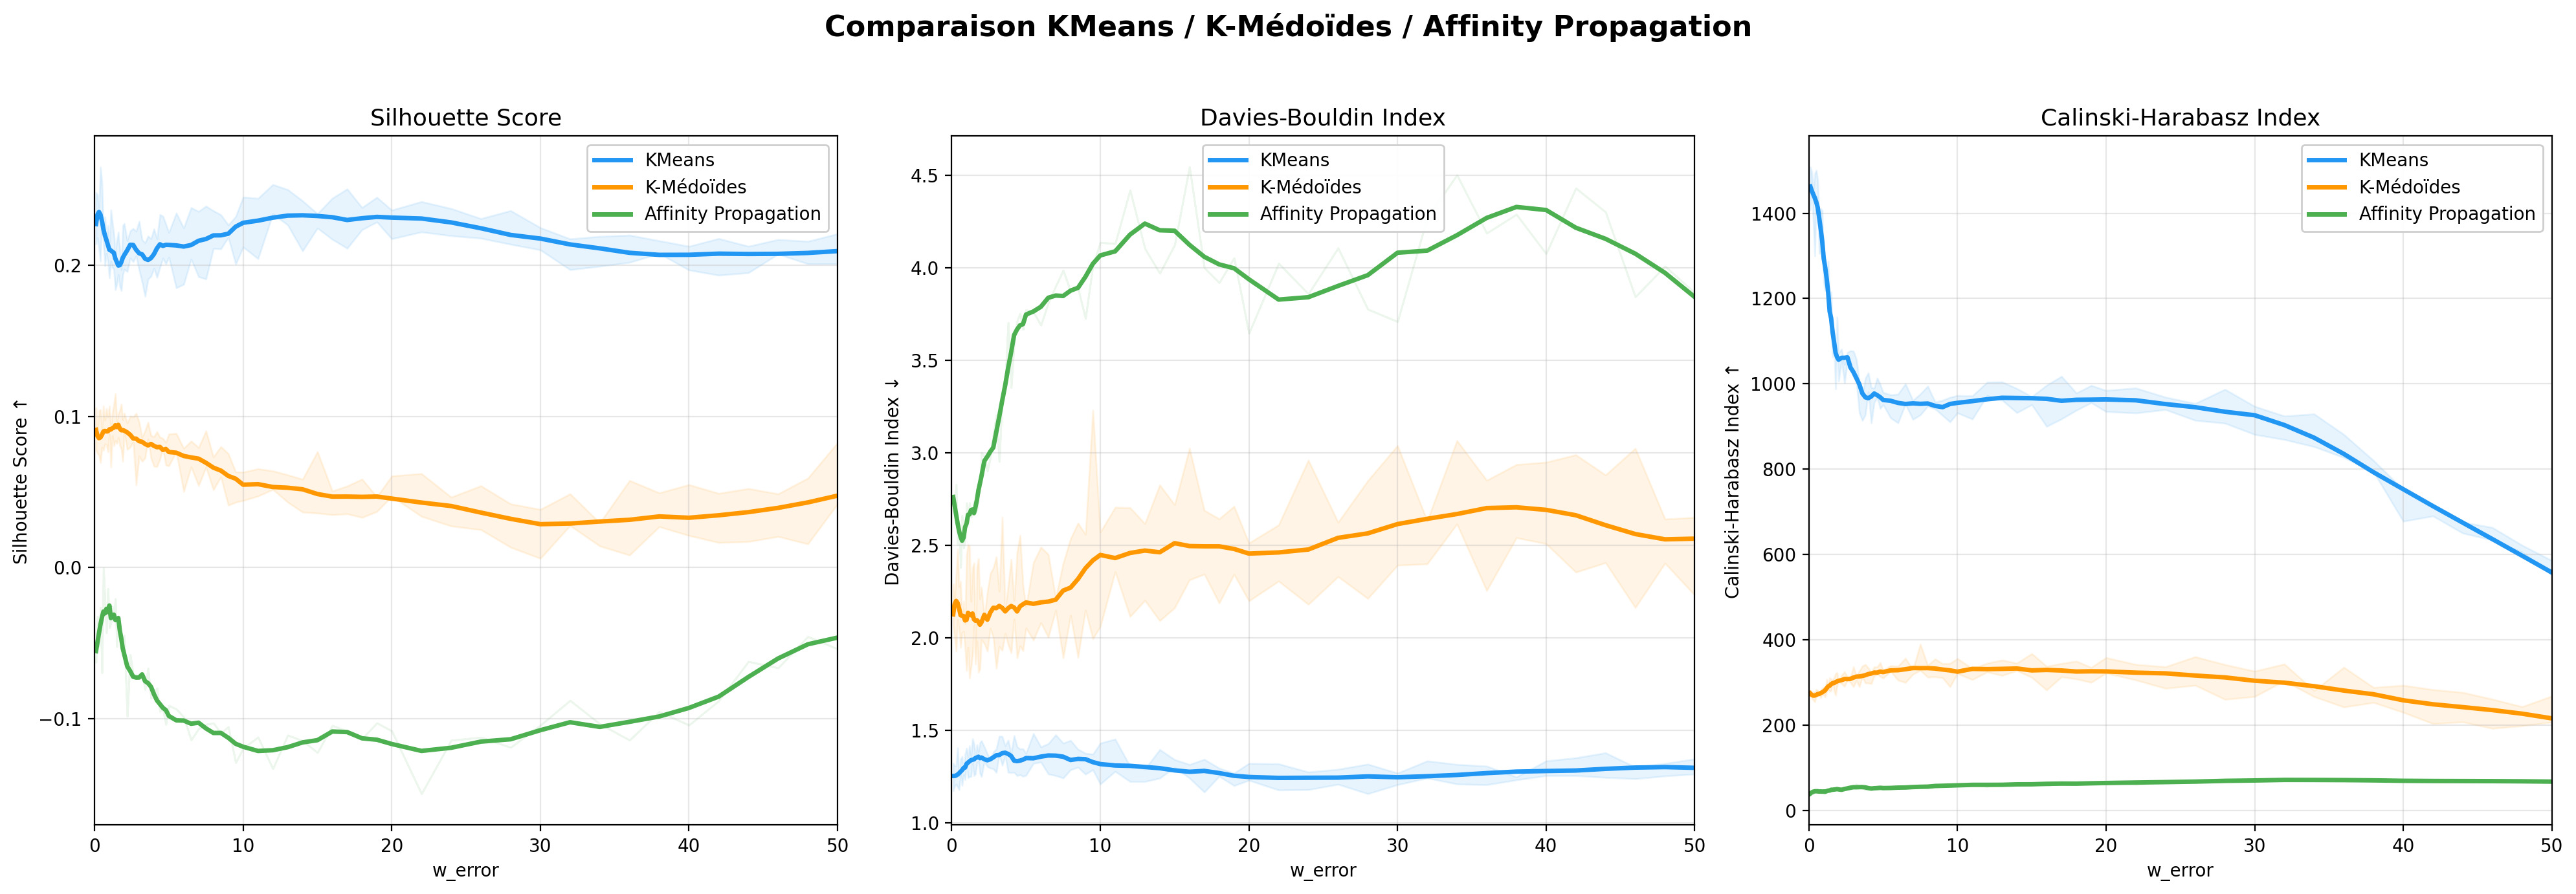
\includegraphics[width=\linewidth, height=0.45\textheight, keepaspectratio]{img/fig3_comparison_algo.jpg}\\
    {\scriptsize Scores de Silhouette par algorithme}

    \vspace{0.15cm}
    \begin{alertblock}{Observation}
        {\small K-Médoïdes et AP \textbf{doublent} le score Silhouette de K-Means grâce à TRACLUS.}
    \end{alertblock}
\end{column}
\end{columns}
\end{frame}

% --- SLIDE : Optimisation de k ---
\begin{frame}{Optimisation de $k$ : compromis topologie / sémantique}
\small
\begin{columns}[T]
\begin{column}{0.55\textwidth}
    \centering
    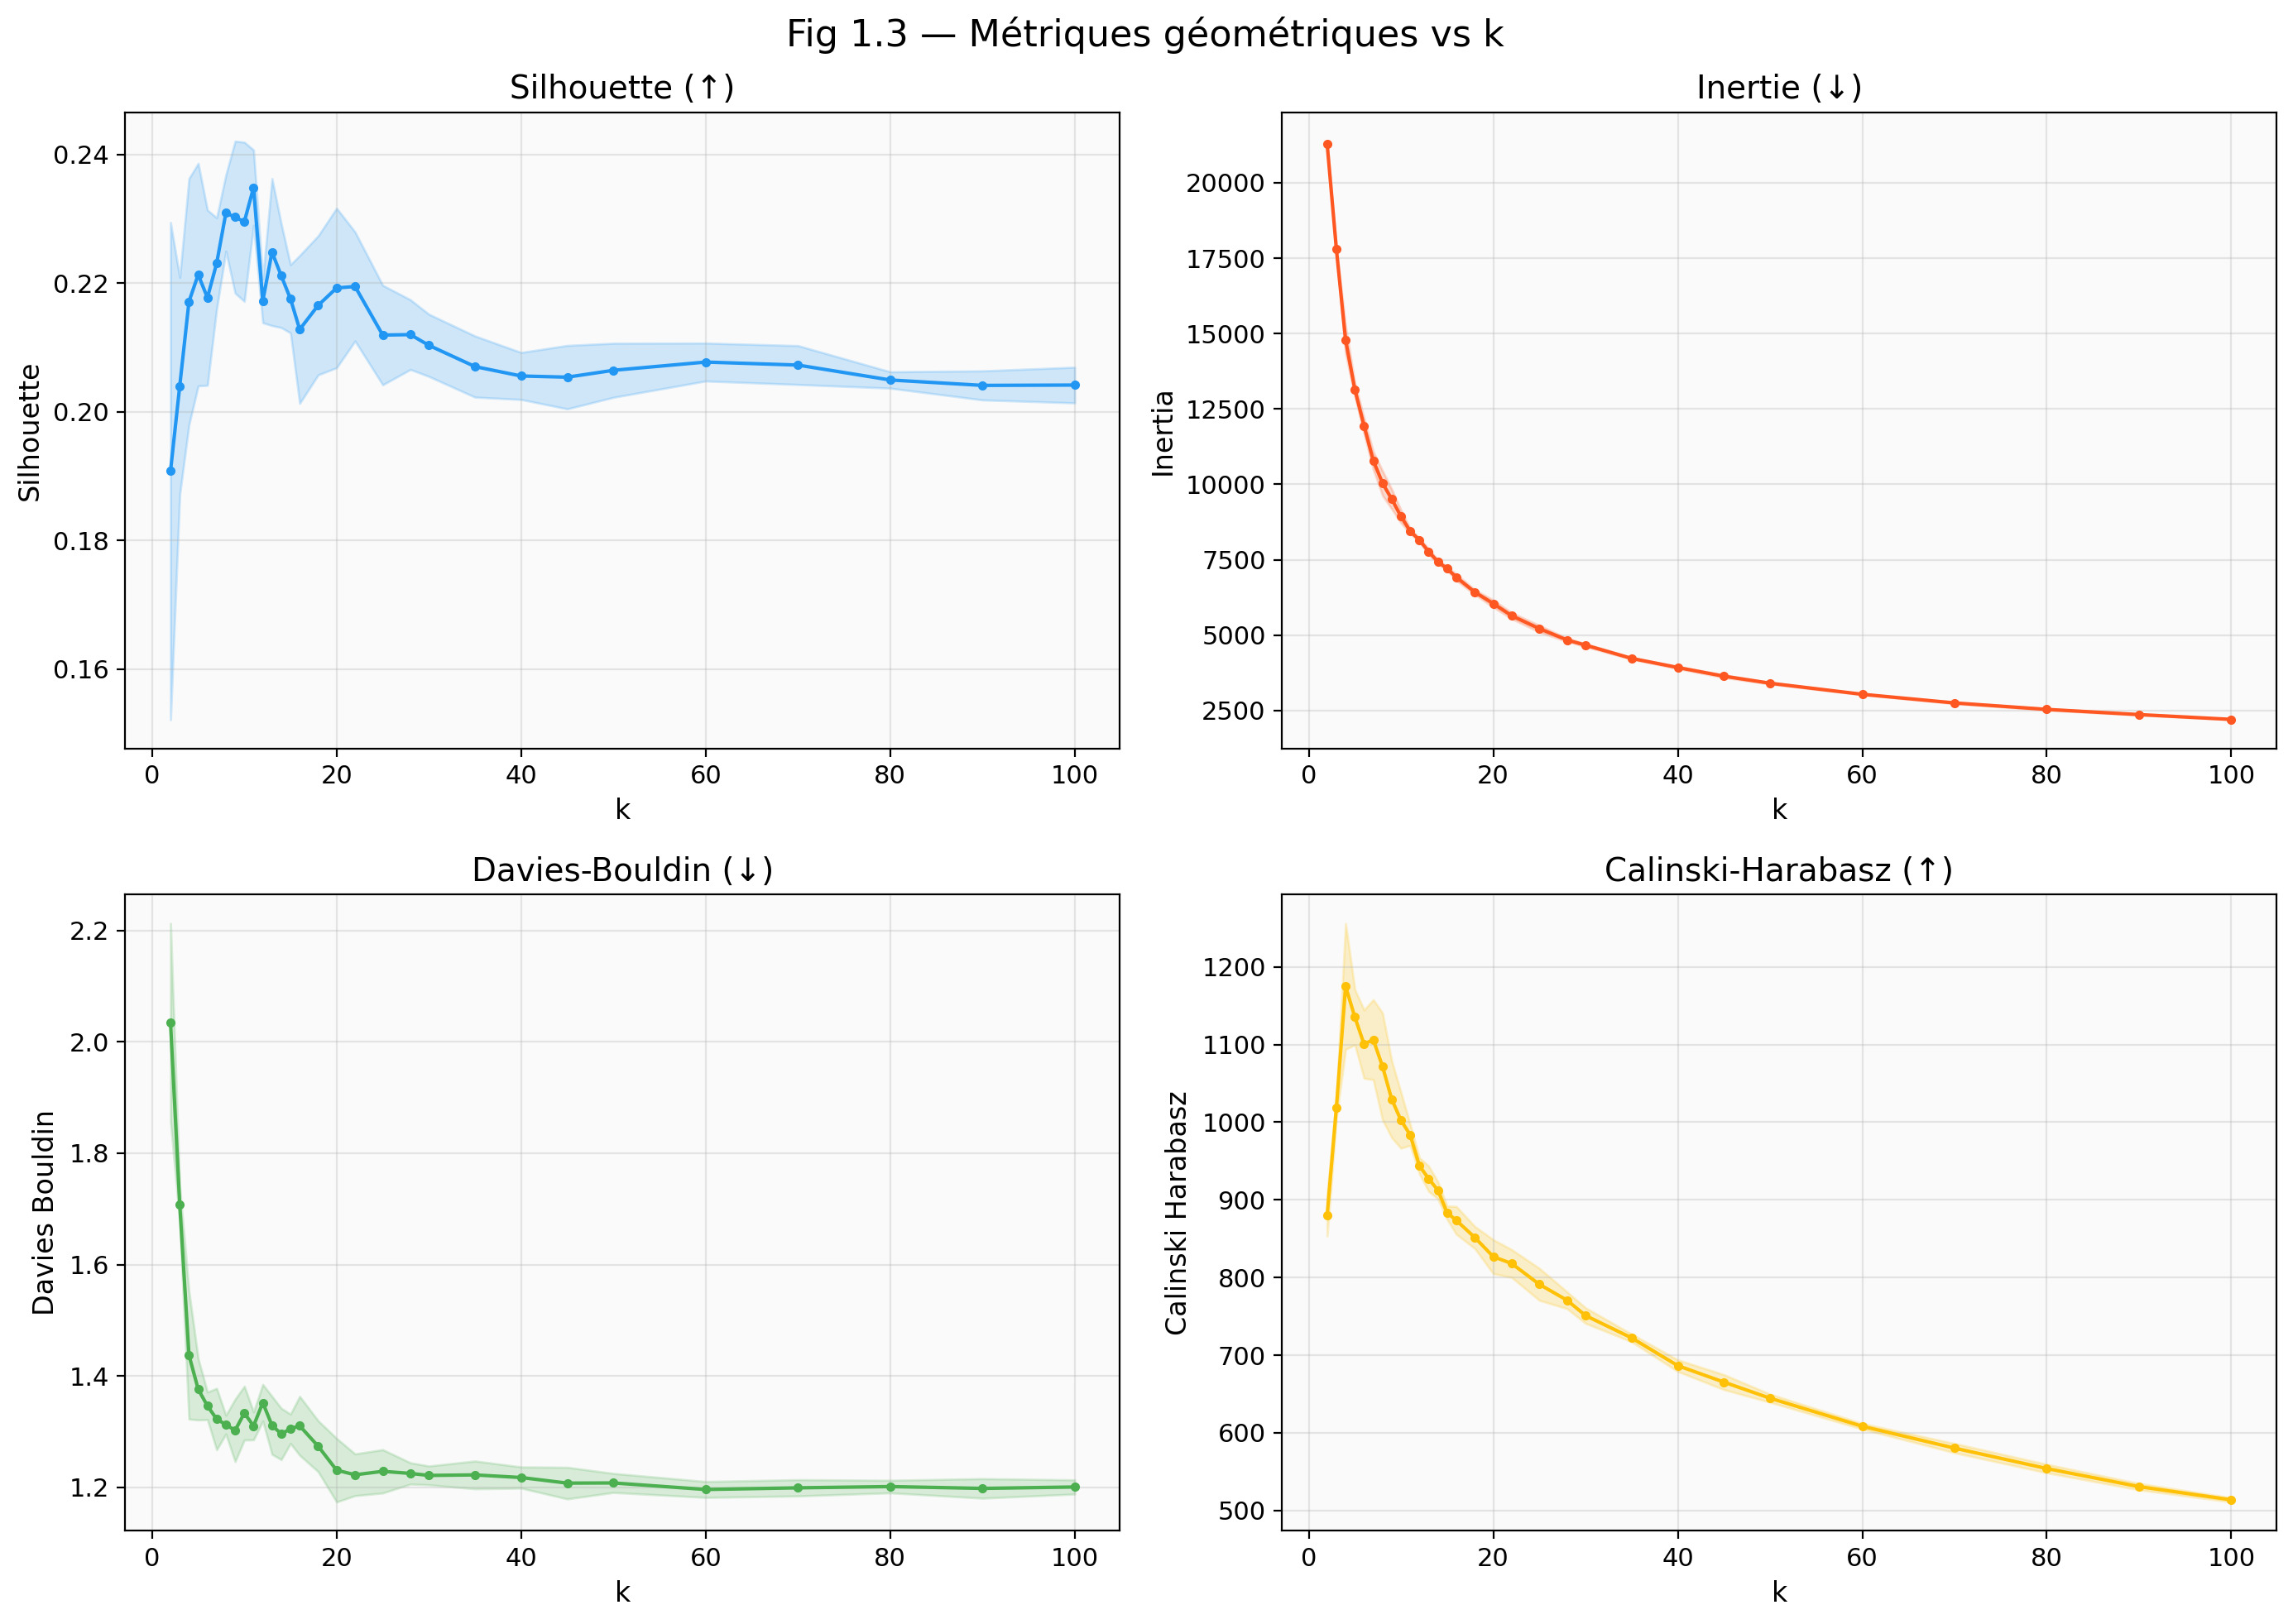
\includegraphics[width=\linewidth, height=0.55\textheight, keepaspectratio]{img/fig1_3_panel_metrics_k.jpg}\\
    {\scriptsize Recherche du $k$ optimal ($k \in [2, 30]$)}
\end{column}
\begin{column}{0.42\textwidth}
    \textbf{Méthode du coude :}
    \begin{itemize}\setlength{\itemsep}{1pt}
        \item \textbf{Davies-Bouldin} : minimum local à $k \approx 10$ \textcolor{dota_green}{\checkmark}
        \item \textbf{Silhouette} : stabilisation en plateau
    \end{itemize}

    \vspace{0.15cm}
    \begin{block}{Validation par PrefixSpan}
        {\small À $k=10$, volume de motifs \textbf{riche mais maîtrisé} : pas d'explosion combinatoire.}
    \end{block}

    \vspace{0.1cm}
    $\Rightarrow$ \textbf{Choix final : $k = 10$ zones}
\end{column}
\end{columns}
\end{frame}

% --- SLIDE : Sensibilité de l'AP ---
\begin{frame}{Sensibilité de l'AP à la taille de l'échantillon}
\small
\begin{columns}[c]
\begin{column}{0.52\textwidth}
    \centering
    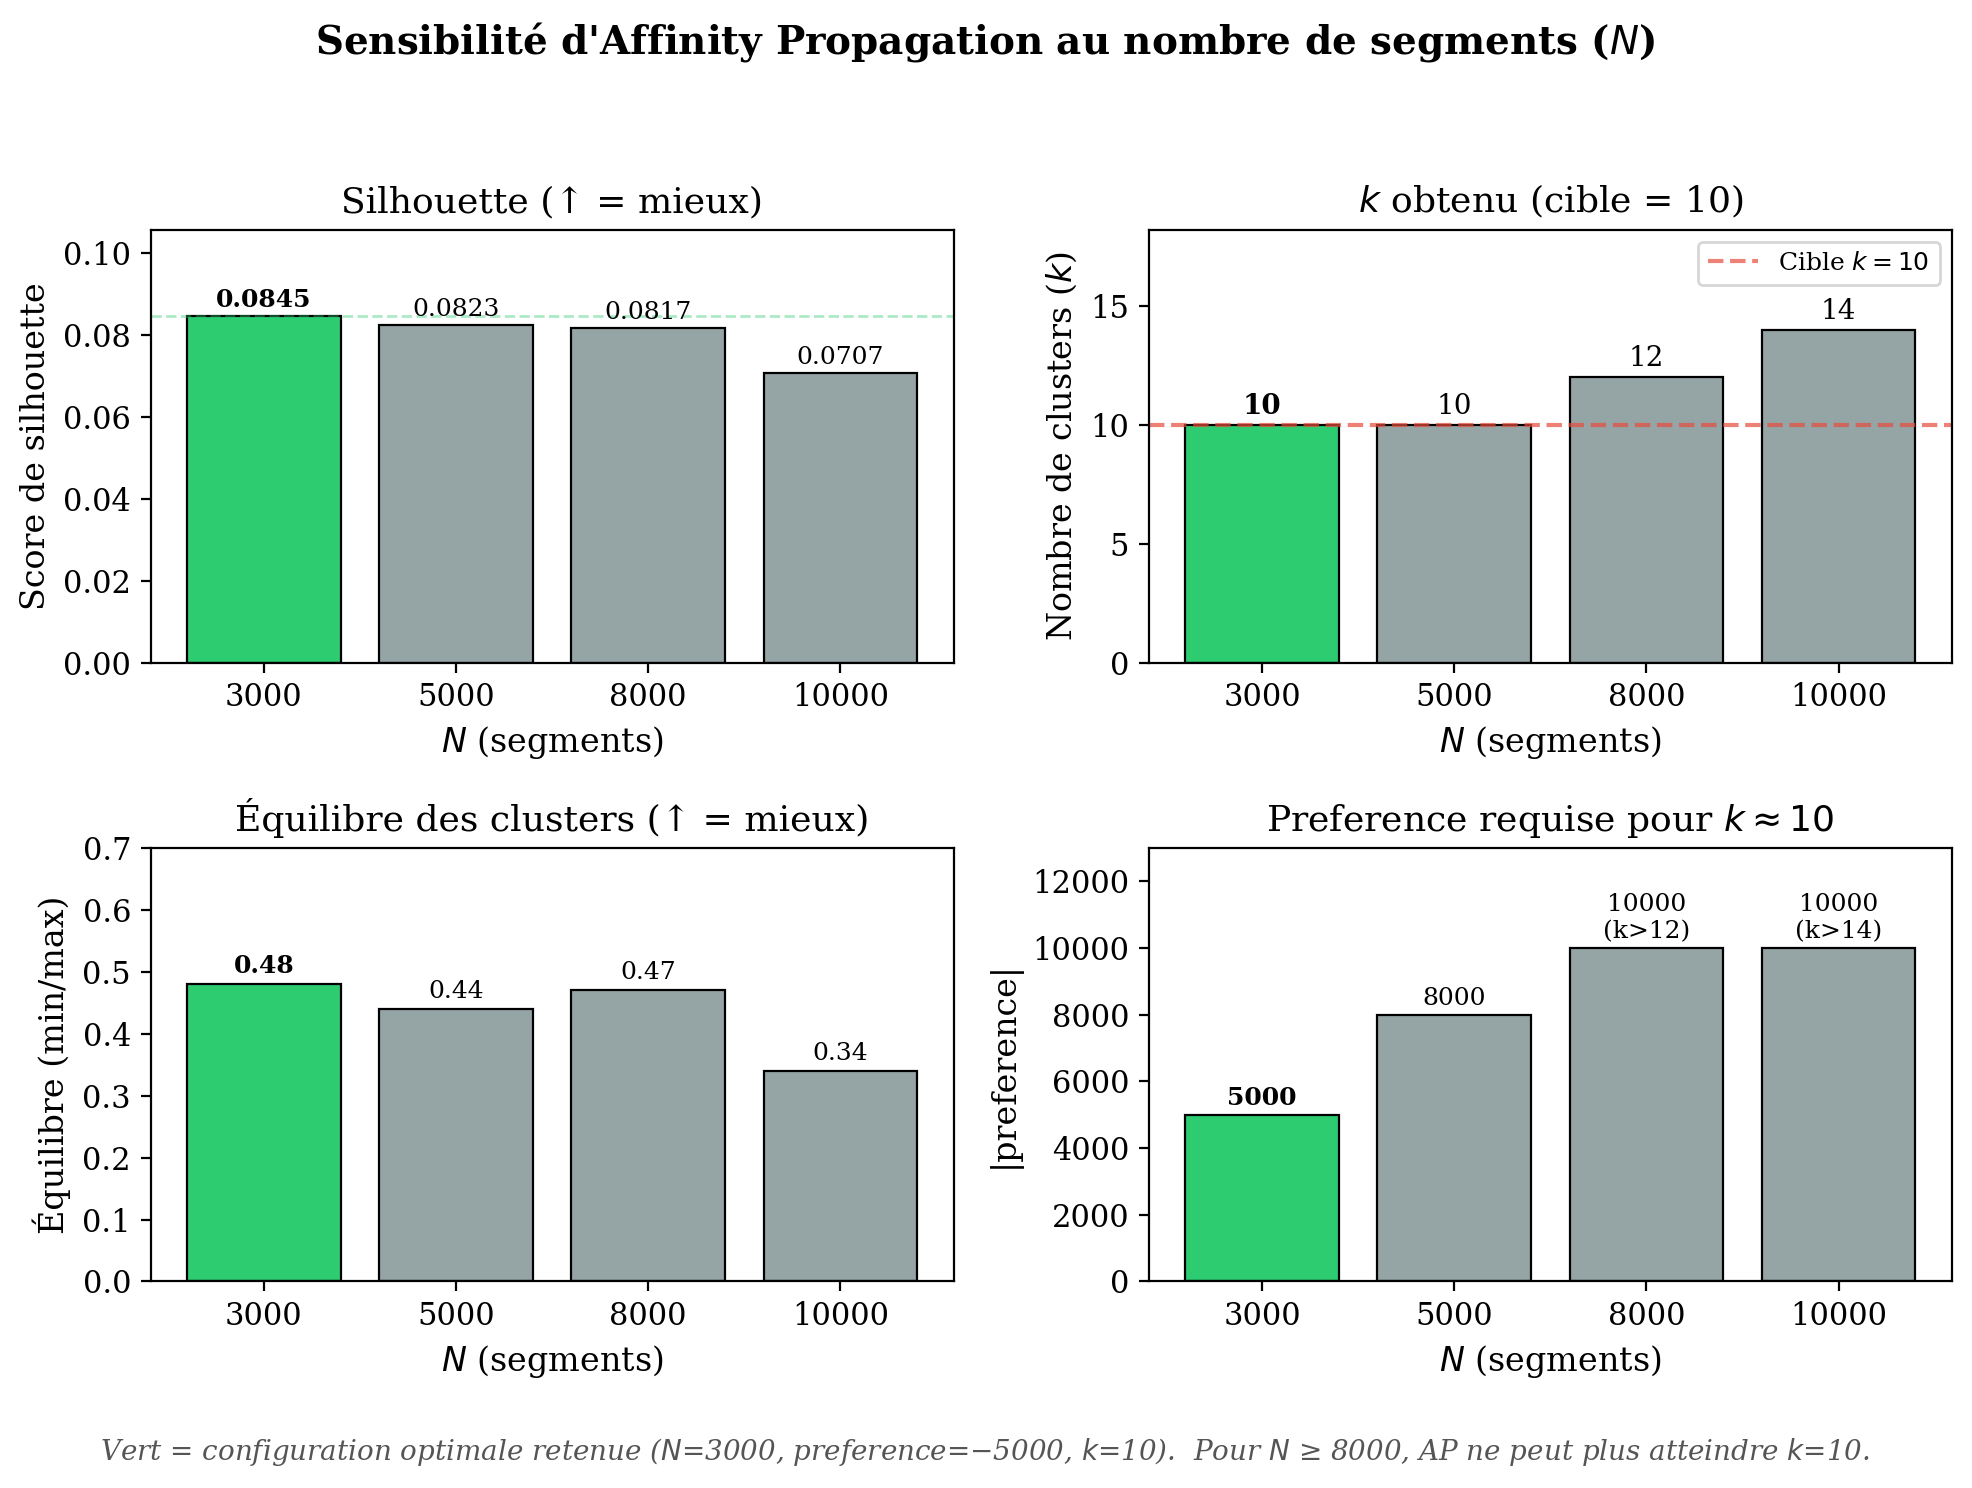
\includegraphics[width=\linewidth, height=0.7\textheight, keepaspectratio]{img/ap_N.jpg}
\end{column}
\begin{column}{0.45\textwidth}
    \begin{itemize}\setlength{\itemsep}{3pt}
        \item \textbf{Passage à l'échelle} : sur-segmentation (12--14 clusters) dès $N \geq 8\,000$
        \item \textbf{Zone de convergence} : $k = 10$ stable pour $N = 3\,000$
    \end{itemize}

    \vspace{0.2cm}
    \begin{block}{Décision technique}
        {\small Sous-échantillonnage à \textbf{$N = 3\,000$ segments} pour un découpage cohérent en 10 zones.}
    \end{block}
\end{column}
\end{columns}
\end{frame}

% --- SLIDE : Benchmark Qualité vs Scalabilité ---
\begin{frame}{Benchmark : qualité vs scalabilité ($k=12$)}
\small
\begin{columns}[c]
\begin{column}{0.52\textwidth}
    \centering
    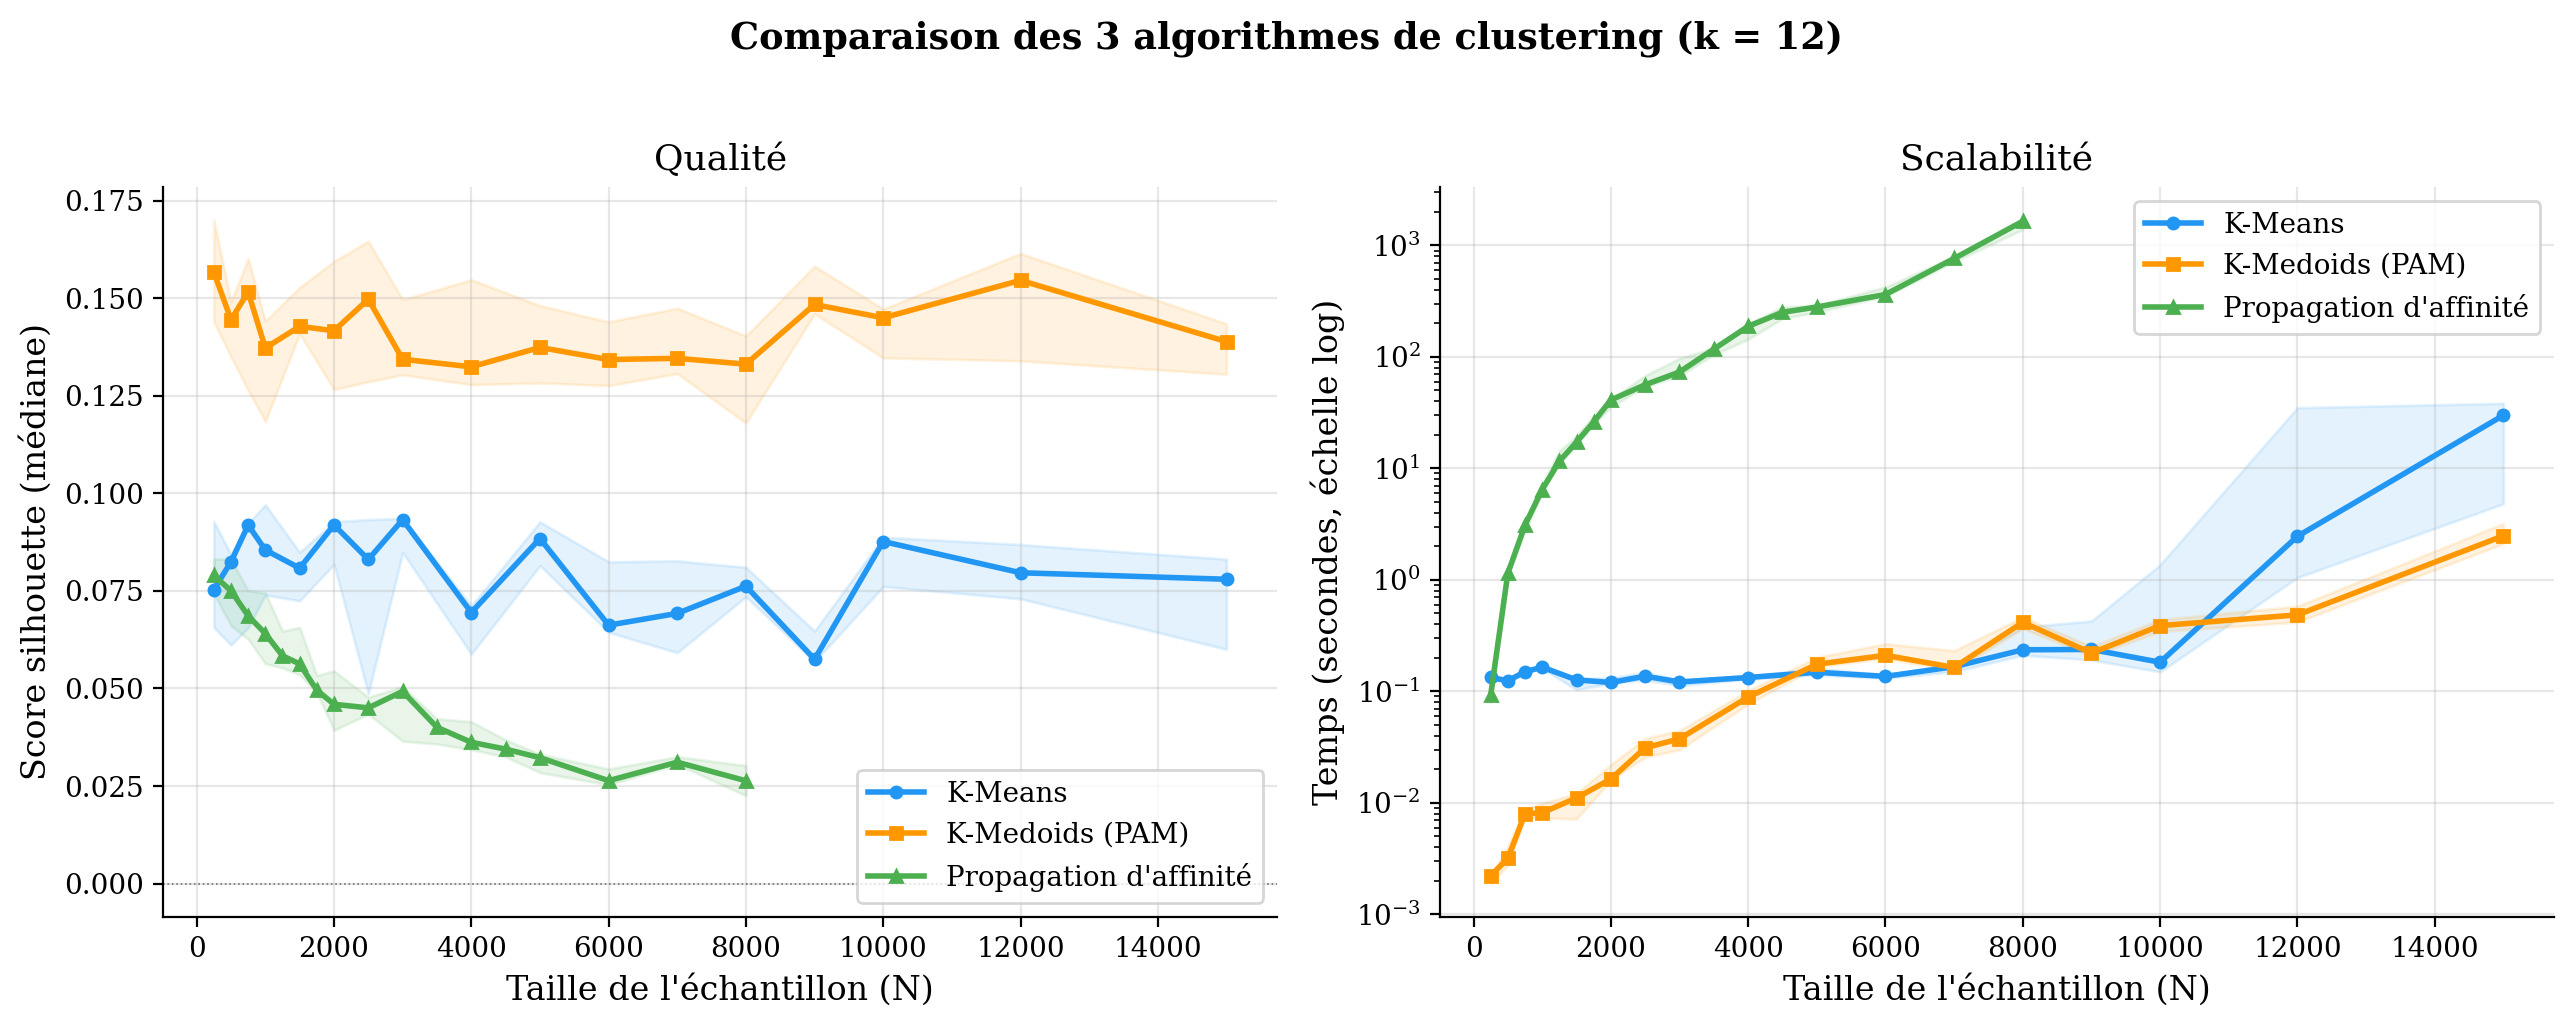
\includegraphics[width=\linewidth, height=0.7\textheight, keepaspectratio]{img/fig3_overview_k12.jpg}
\end{column}
\begin{column}{0.45\textwidth}
    \begin{block}{Qualité (Silhouette)}
        {\small\begin{itemize}\setlength{\itemsep}{1pt}
            \item \textbf{K-Médoïdes} domine (médiane $\approx 0.15$)
            \item \textbf{AP} : instable si $N > 8\,000$
        \end{itemize}}
    \end{block}

    \vspace{0.1cm}
    \begin{block}{Scalabilité (temps)}
        {\small\begin{itemize}\setlength{\itemsep}{1pt}
            \item \textbf{K-Means / K-Médoïdes} : quasi linéaires
            \item \textbf{AP} : $\mathcal{O}(N^2)$, prohibitif $> 4\,000$ seg.
        \end{itemize}}
    \end{block}

    \vspace{0.1cm}
    {\footnotesize Benchmark à $k=12$ fixé. En production, l'AP converge vers $k=10$.}
\end{column}
\end{columns}
\end{frame}

% --- SLIDE : Paradoxe K-Médoïdes + Choix final AP ---
\begin{frame}{Pourquoi l'AP malgré le K-Médoïdes ?}
\small
\begin{columns}[c]
\begin{column}{0.55\textwidth}
    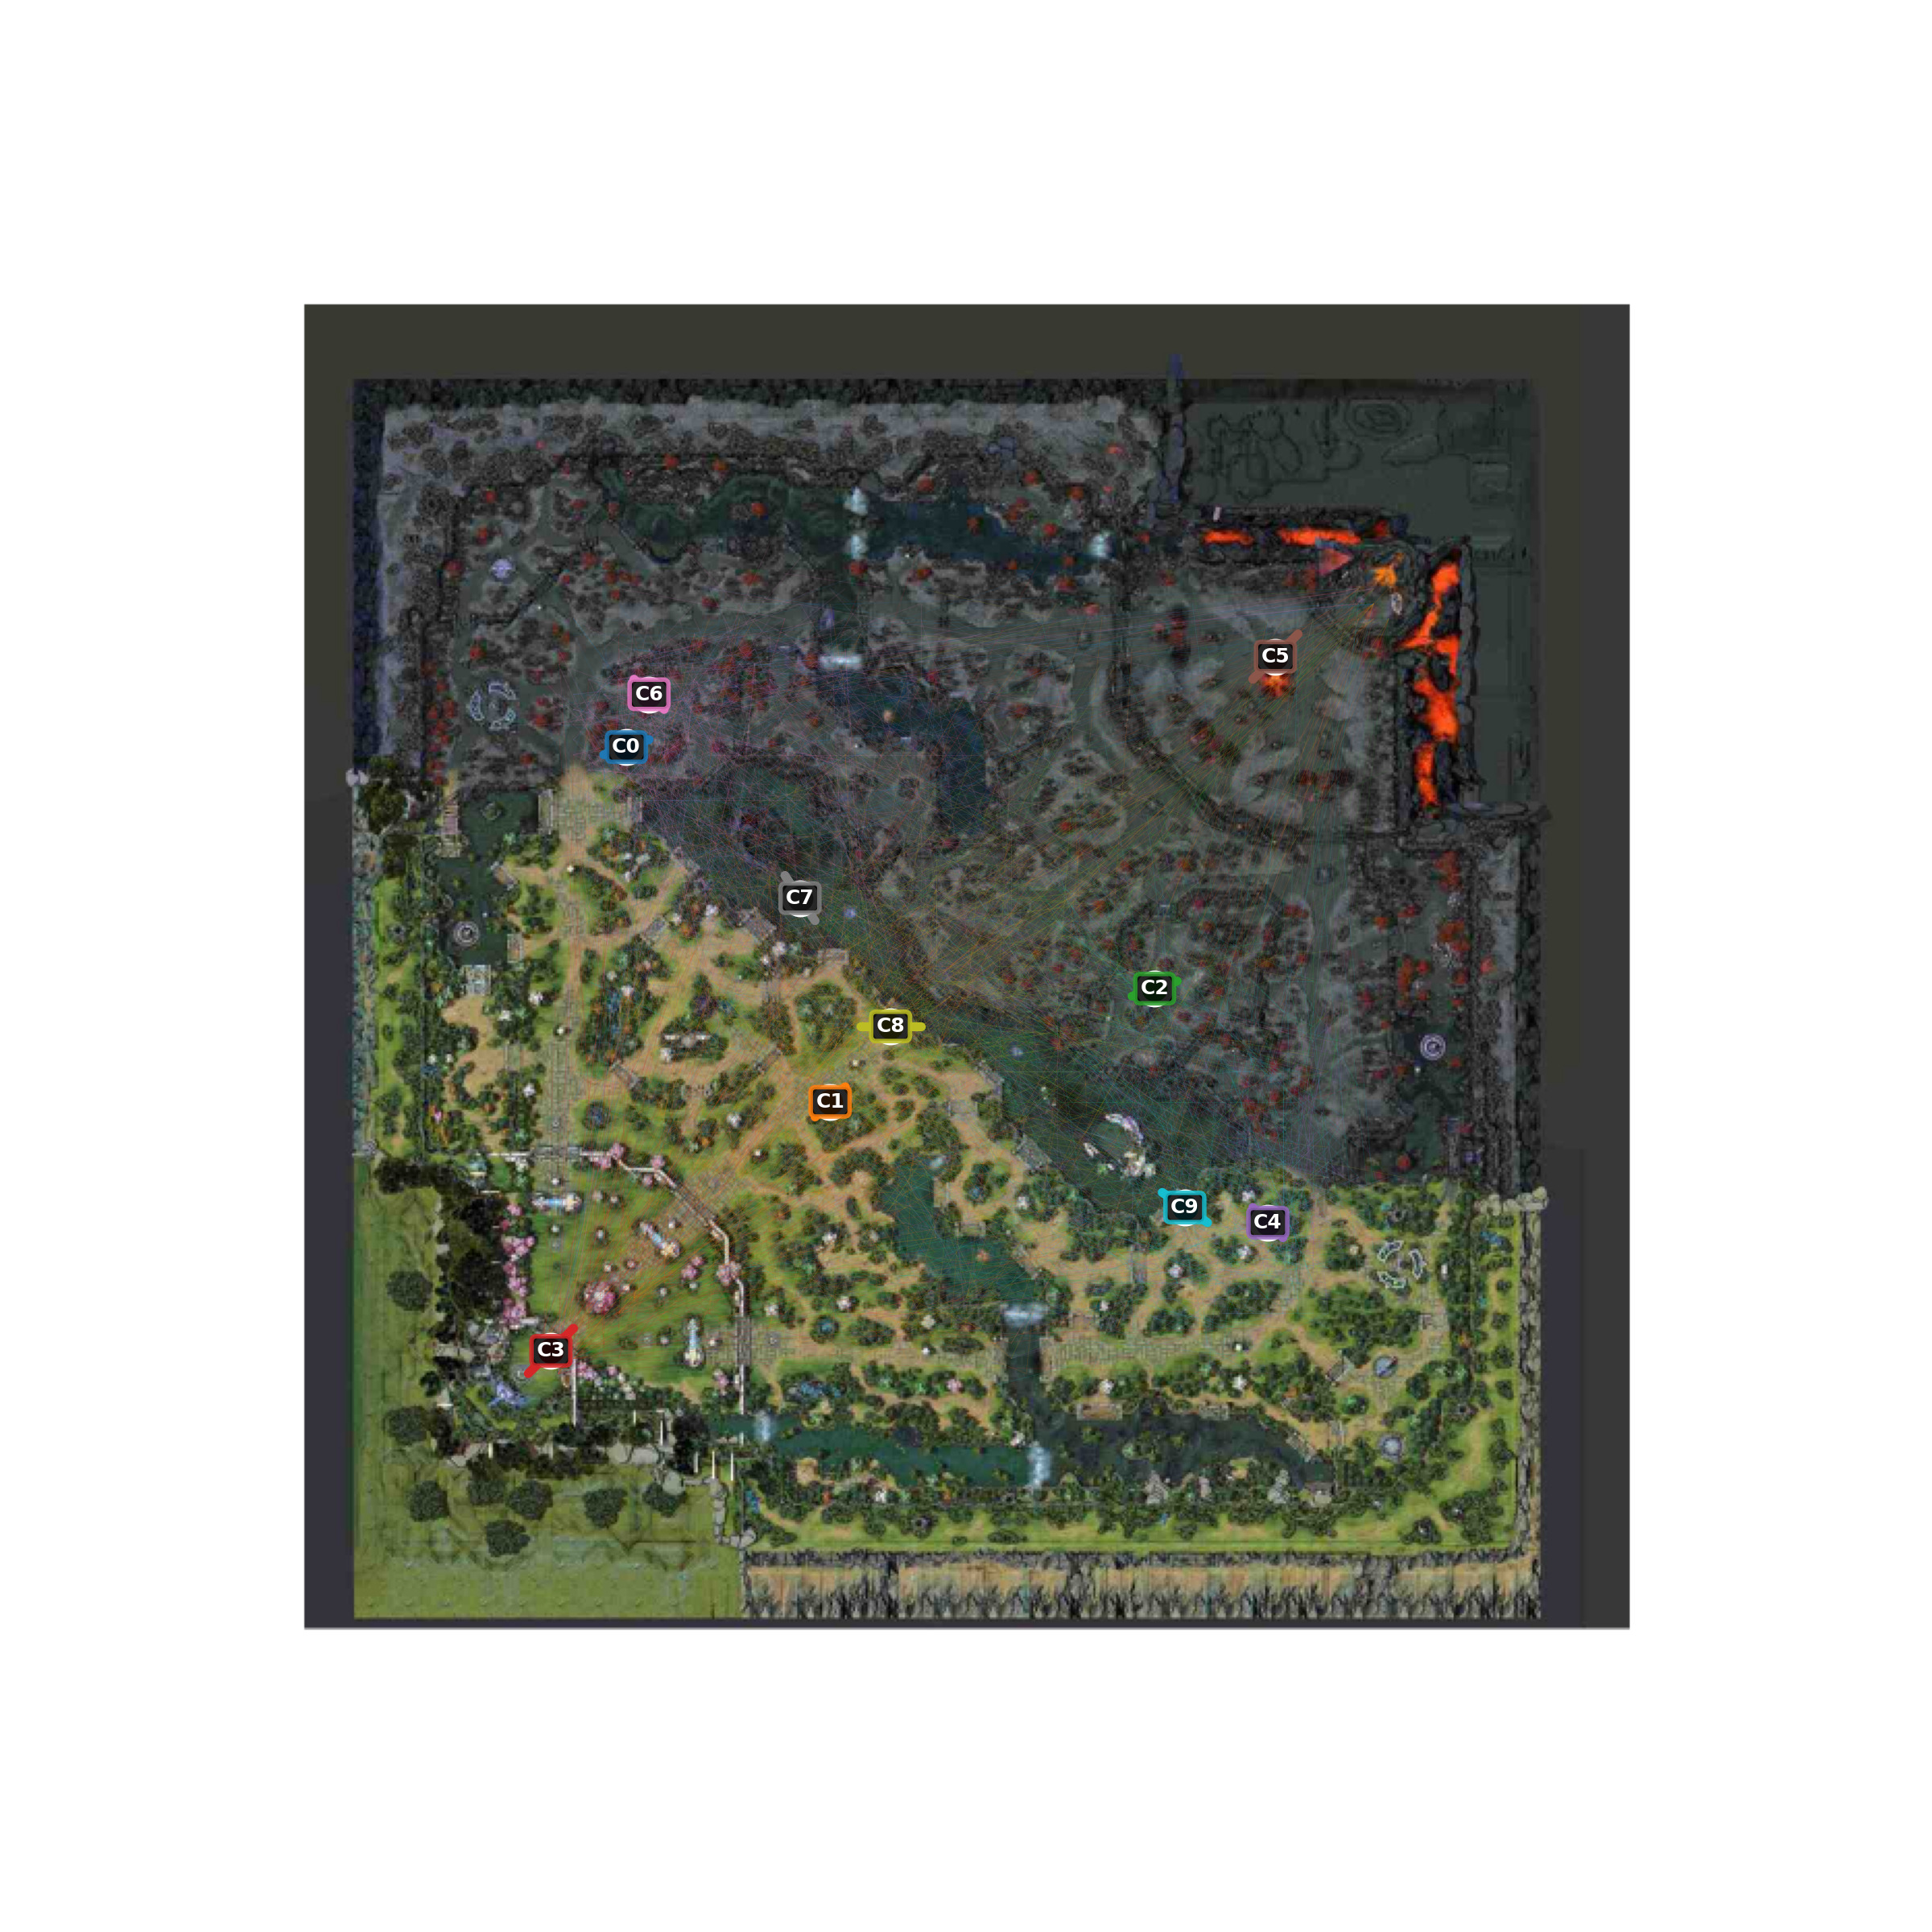
\includegraphics[width=\linewidth, height=0.82\textheight, keepaspectratio]{img/fig3_1_clusters_map.jpg}\\
    {\scriptsize Les 10 macro-zones découvertes par l'AP}
\end{column}
\begin{column}{0.43\textwidth}
    \textbf{\textcolor{dota_accent}{Le paradoxe K-Médoïdes :}}
    \begin{itemize}\setlength{\itemsep}{1pt}
        \item Meilleur Silhouette, mais \textbf{doublons} : 2 centres à $< 5$ unités
        \item Zones entières ignorées (Top Lane)
        \item Bon score $\neq$ cohérence géographique
    \end{itemize}

    \vspace{0.15cm}
    \textbf{\textcolor{dota_green}{Paramétrage AP retenu :}}
    \begin{itemize}\setlength{\itemsep}{1pt}
        \item $N = 3\,000$ segments
        \item Damping $= 0.7$
        \item Préférence $= -5\,000$ ($\to k \approx 10$)
    \end{itemize}

    \vspace{0.1cm}
    \begin{alertblock}{Verdict}
    {\small AP = seul algo avec \textbf{couverture complète} de la carte, servant d'\textbf{alphabet} pour PrefixSpan.}
    \end{alertblock}
\end{column}
\end{columns}
\end{frame}

\begin{frame}{PrefixSpan — Extraction de motifs séquentiels}
    \begin{columns}
        \column{0.6\textwidth}
        \textbf{Principe :}
        \begin{itemize}
            \item Trouver les sous-séquences d'états fréquentes
            \item Approche par \textit{pattern growth}
        \end{itemize}
        \vspace{0.5em}
        \textbf{Paramètres :}
        \begin{itemize}
            \item minSupport : $0.2 =  20 \%$
            \item maxLength : 5 
        \end{itemize}
        
        \column{0.4\textwidth}
        % Diagramme du pipeline ou pseudo-code simplifié
        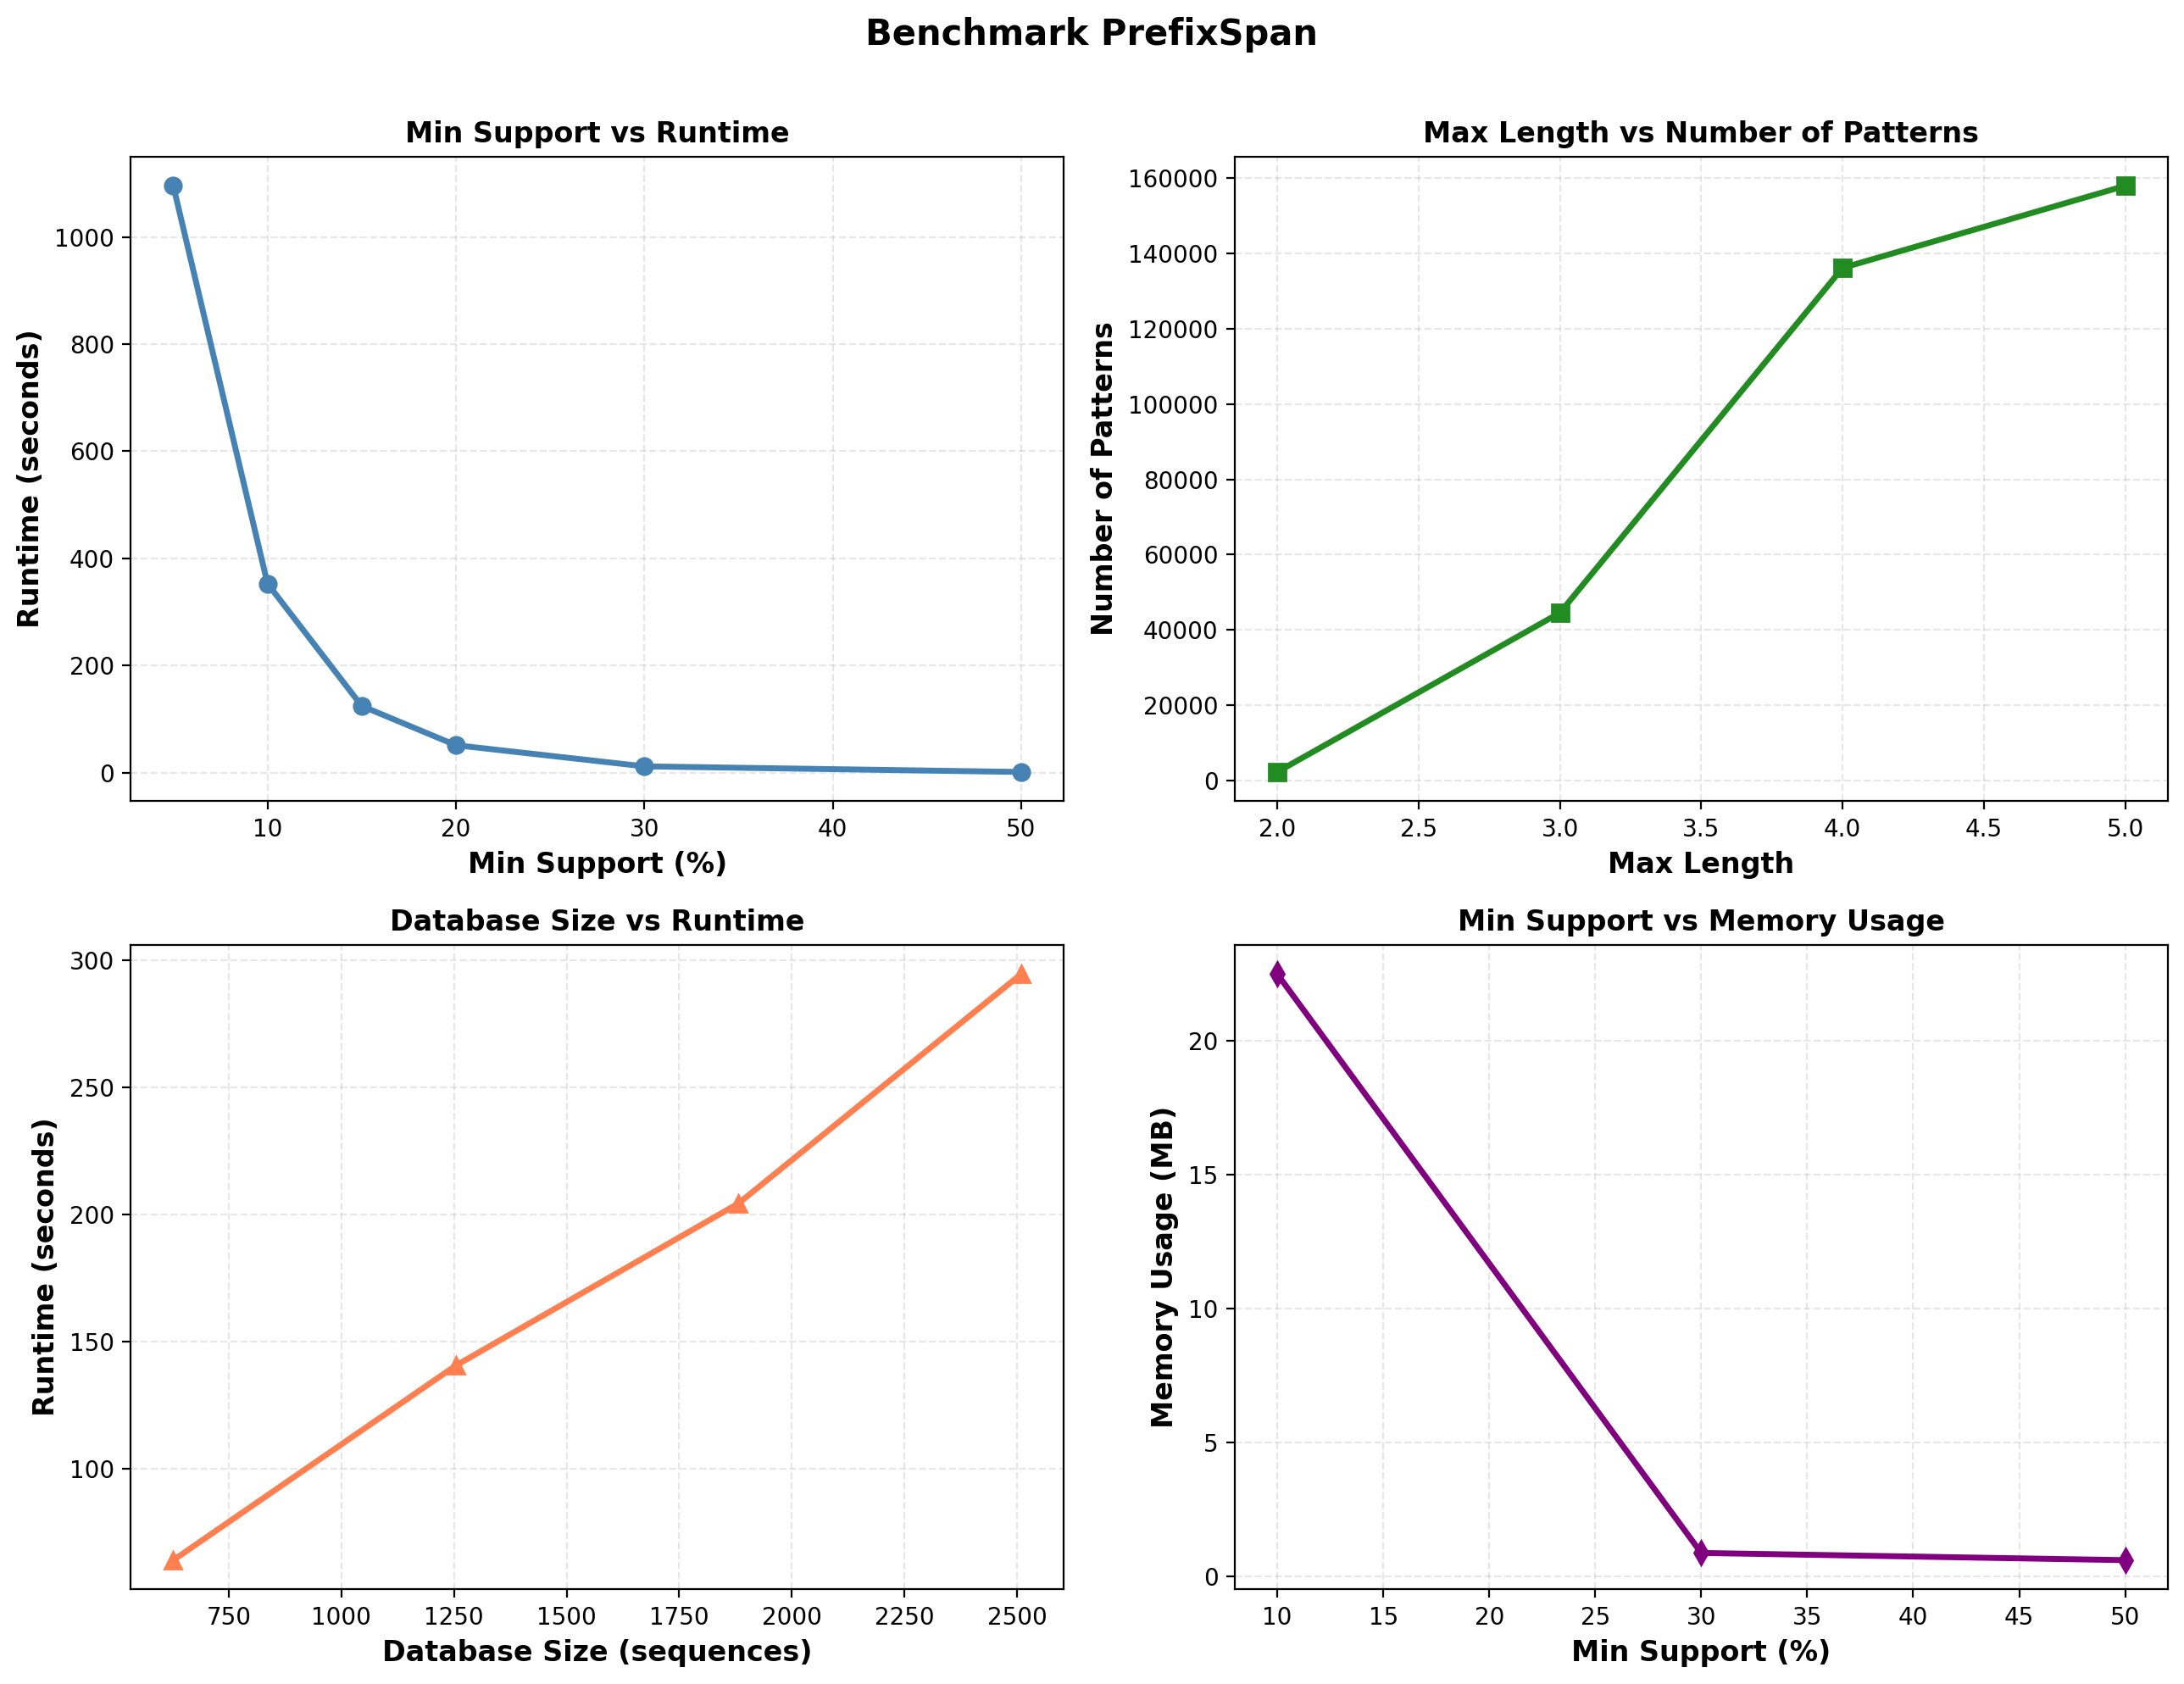
\includegraphics[width=\linewidth, height=0.7\textheight, keepaspectratio]{img/prefixspan_benchmark.jpg}
    \end{columns}
\end{frame}

\begin{frame}{PrefixSpan — Comment trouver des schémas de jeu récurrents ?}
\small
\begin{columns}[T]
\begin{column}{0.40\textwidth}
    \textbf{Principe :}
    \begin{itemize}\setlength{\itemsep}{6pt}
        \item Chaque trajectoire compressée est une \textbf{suite de clusters} (ex: 14, 68, 83\ldots)
        \item On cherche les \textbf{enchaînements de clusters} qui apparaissent dans beaucoup de séquences
        \item On part d'un cluster fréquent, puis on regarde ce qui \textbf{suit} dans les séquences concernées
        \item Si le prolongement est aussi fréquent, on \textbf{continue} ; sinon on \textbf{s'arrête} 
    \end{itemize}

    \vspace{0.25cm}
    {\footnotesize\textbf{Params :} support $\geq 20\%$, longueur $\leq 5$}
\end{column}
\begin{column}{0.56\textwidth}
    \centering
    \textbf{Pattern Growth — arbre d'exploration}\\[0.2cm]
    \begin{tikzpicture}[
        every node/.style={font=\footnotesize},
        level 1/.style={sibling distance=2.2cm, level distance=1.2cm},
        level 2/.style={sibling distance=1.4cm, level distance=1.2cm},
        level 3/.style={sibling distance=1.2cm, level distance=1.1cm},
        bag/.style={draw, rounded corners, fill=dota_dark!10, minimum width=1.1cm, minimum height=0.55cm, align=center},
        freq/.style={bag, fill=dota_green!30, draw=dota_green!70!black},
        stop/.style={bag, fill=red!15, draw=red!50, dashed},
        arr/.style={draw, thick},
        sup/.style={font=\scriptsize\color{gray}}
    ]
    \node[bag, fill=dota_gold!20] (root) {Base}
        child { node[freq] (n14) {14}
            child { node[freq] (n1468) {14,68}
                child { node[stop] (n146883) {14,68}
                }
                child { node[stop] (n146836) {14,68,36}
                }
            }
        }
        child { node[freq] (n68) {68}
            child { node[freq] (n6836) {68,36}
            }
        }
        child { node[freq] (n91) {91}
            child { node[freq] (n9168) {91,68}
            }
        };
    % Flèches manuelles pour éviter les décalages
    \draw[arr, ->] (root) -- node[left, sup] {sup=2} (n14);
    \draw[arr, ->] (root) -- node[left, sup] {sup=3} (n68);
    \draw[arr, ->] (root) -- node[right, sup] {sup=1} (n91);
    \draw[arr, ->] (n14) -- node[left, sup] {2} (n1468);
    \draw[arr, ->] (n1468) -- node[left, sup] {1} (n146883);
    \draw[arr, ->] (n1468) -- node[right, sup] {1} (n146836);
    \draw[arr, ->] (n68) -- node[right, sup] {2} (n6836);
    \draw[arr, ->] (n91) -- node[right, sup] {1} (n9168);
    \end{tikzpicture}

    \vspace{0.2cm}
    {\scriptsize
    \colorbox{dota_green!20}{\strut~Fréquent~} = support $\geq$ seuil \quad
    \colorbox{red!10}{\strut~Stop~} = trop rare, on arrête}
\end{column}
\end{columns}
\end{frame}

\begin{frame}{Résultats — Motifs et graphe de transitions}
    \begin{columns}
        \column{0.45\textwidth}
        \small
        \begin{tabular}{|c|c|}
            \hline
            \textbf{Motif} & \textbf{Sup.} \\
            \hline
            14 $\rightarrow$ 68 & 22 \\
            91 $\rightarrow$ 68 & 24 \\
            91 $\rightarrow$ 36 & 21 \\
            68 $\rightarrow$ 83 & 19 \\
            \hline
        \end{tabular}
        \vspace{0.4em}
        
        \textbf{Interprétation :} Clusters 14, 68, 91 = hubs stratégiques
        
        \column{0.55\textwidth}
        \centering
        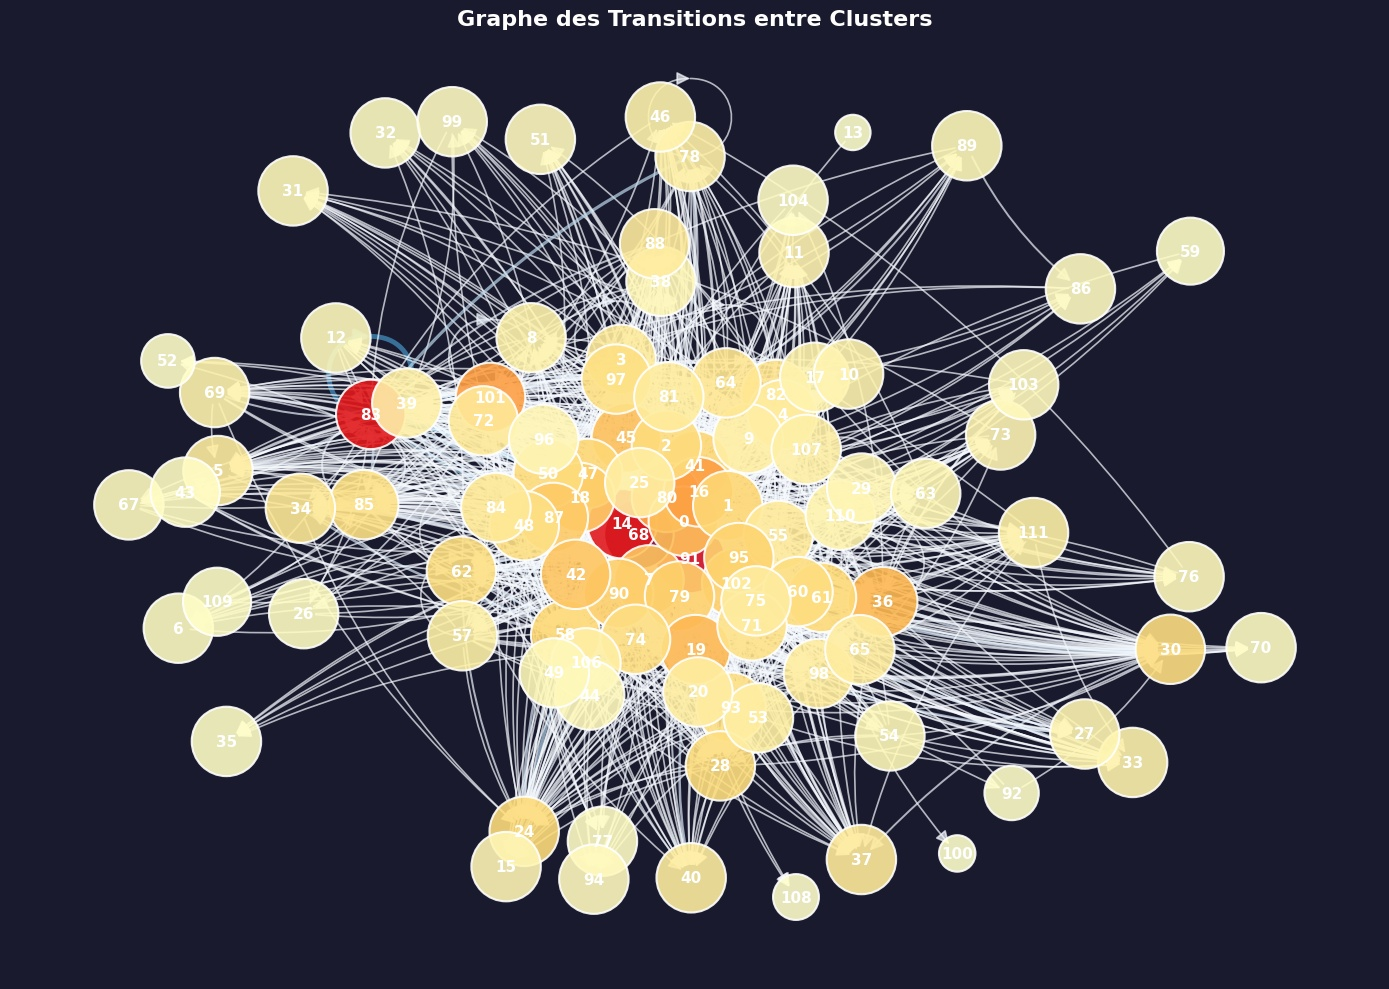
\includegraphics[width=\linewidth, height=0.62\textheight, keepaspectratio]{img/Graphe_des_Transitions.jpg}\\[0.15cm]
        {\scriptsize $w_{error}{=}12$ \quad AP: damping${=}0.9$, max\_iter${=}400$, max\_files${=}5$\\
        PrefixSpan: min\_support${=}0.2$, max\_len${=}5$}
    \end{columns}
\end{frame}

\begin{frame}{Résultats — Stratégies découvertes sur la carte}
\small
\begin{columns}[T]
\begin{column}{0.48\textwidth}
    \centering
    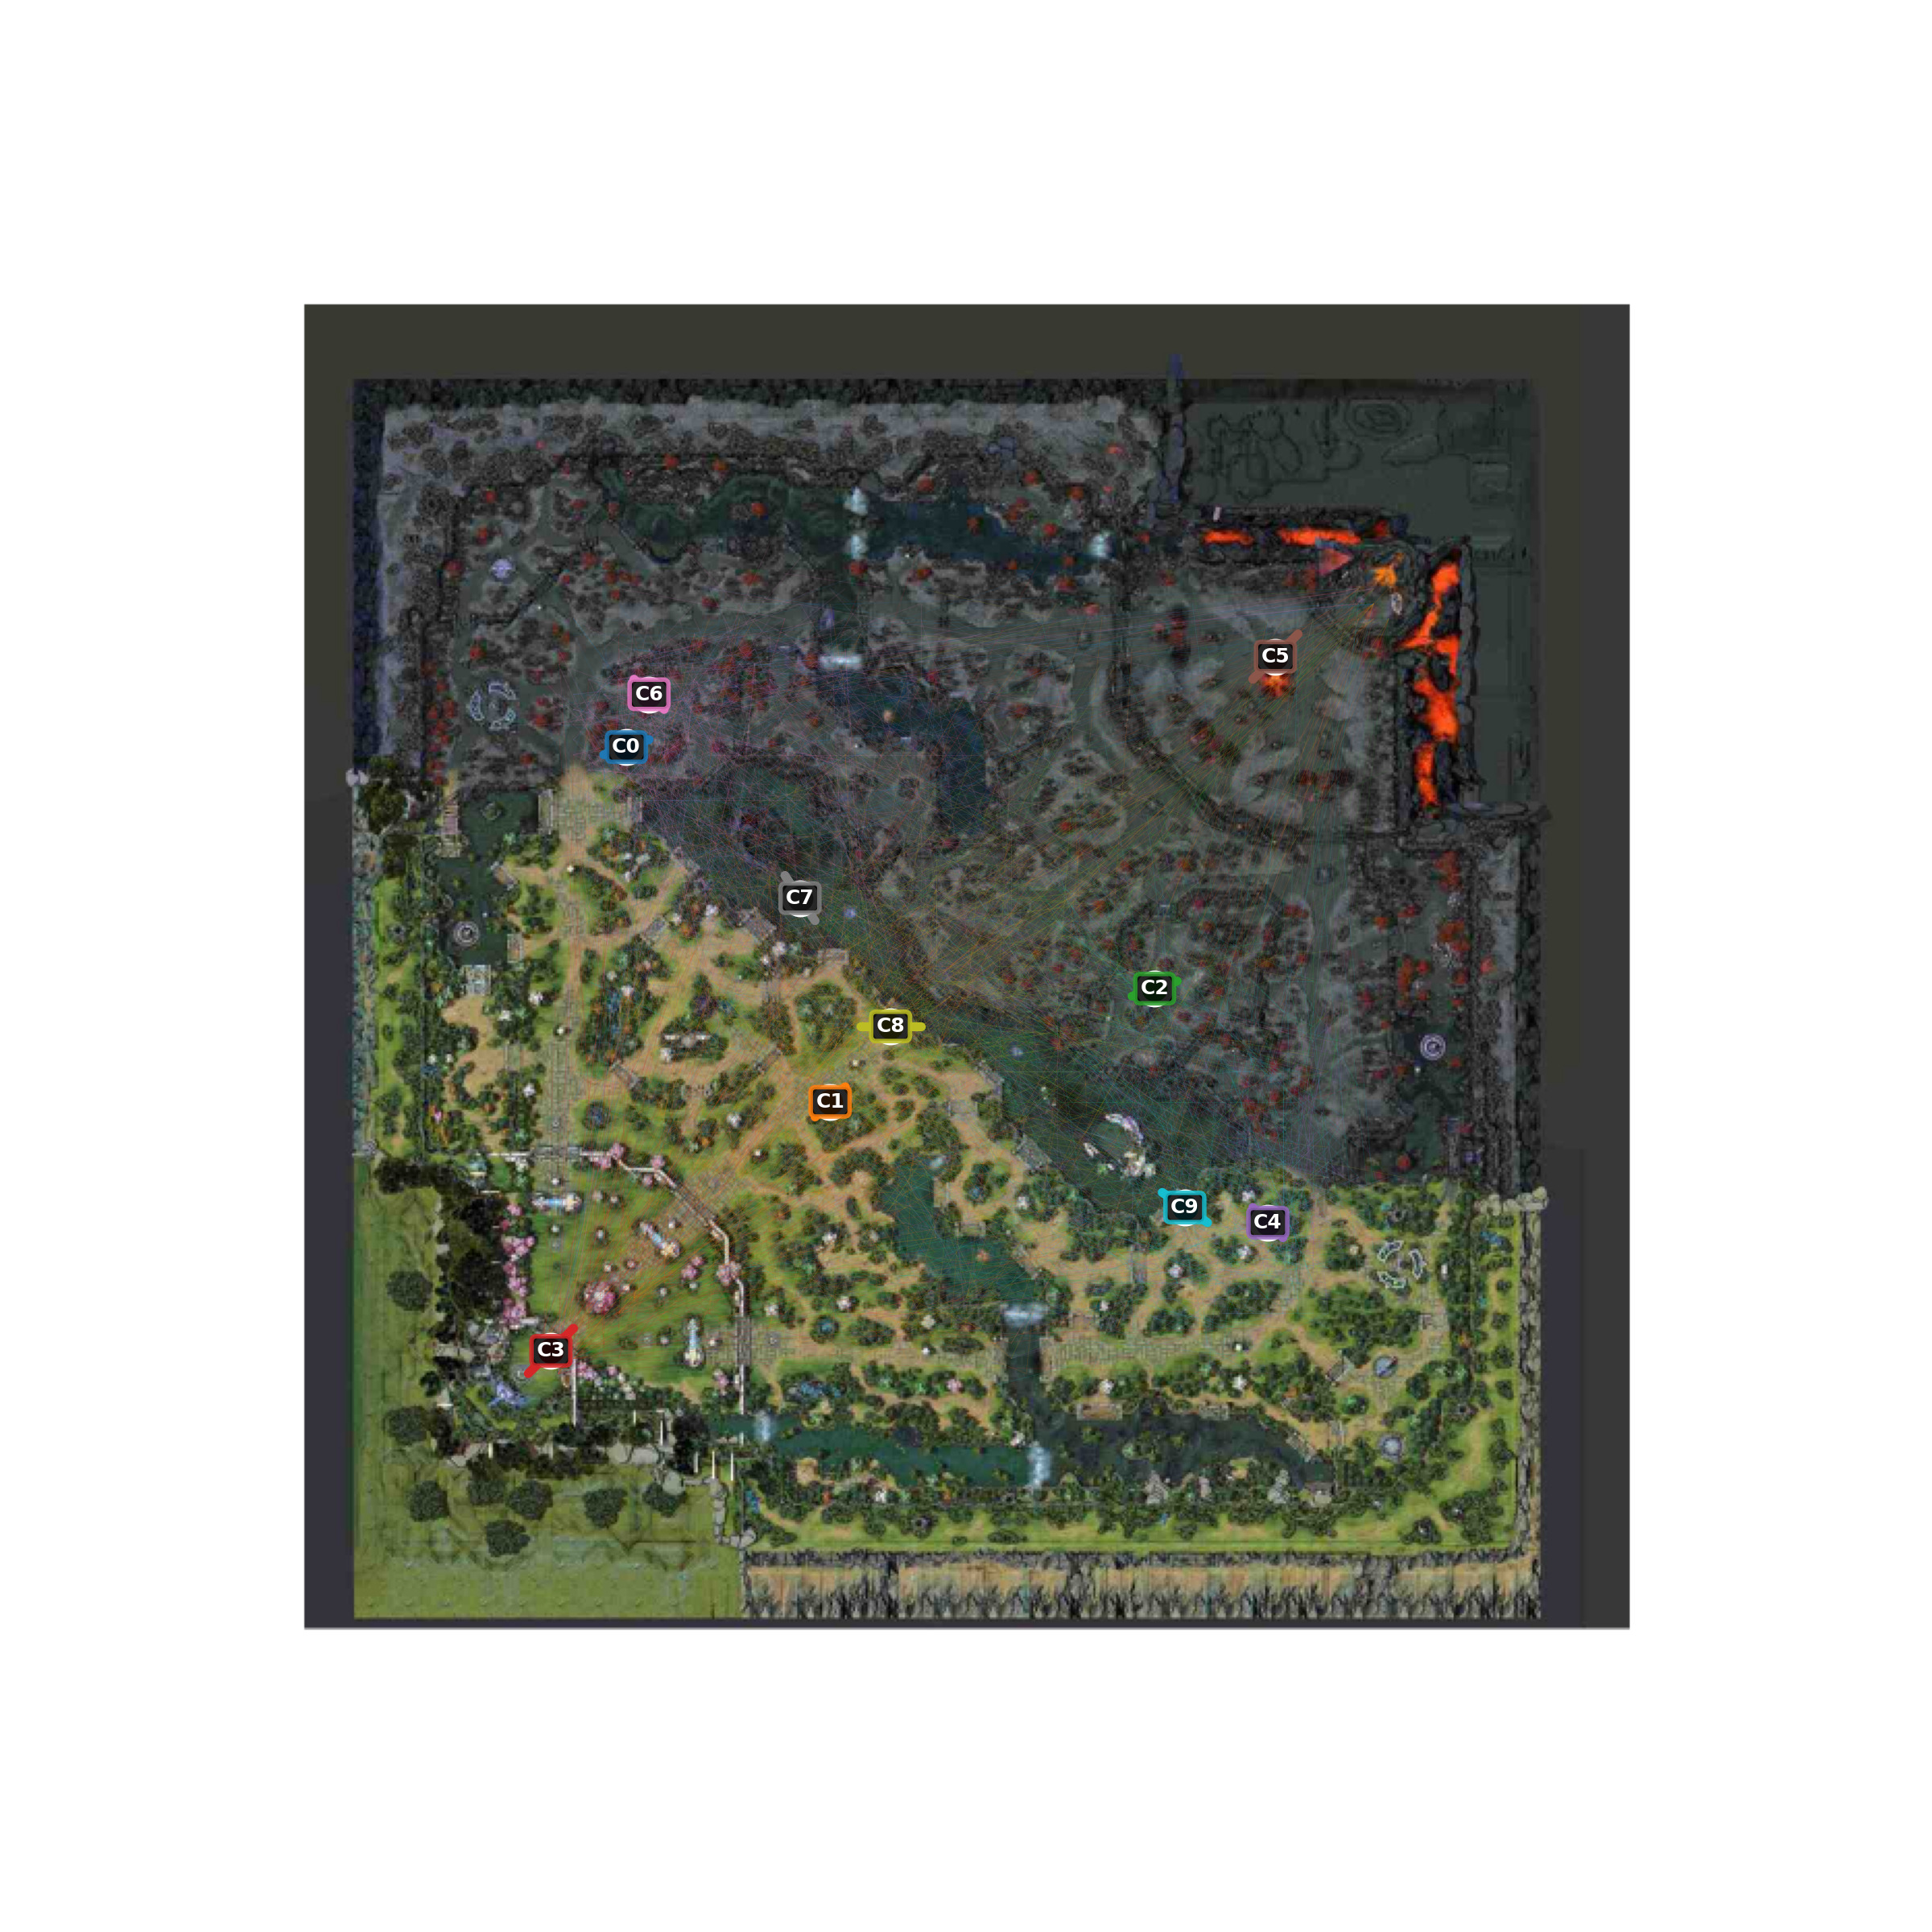
\includegraphics[width=\linewidth, height=0.8\textheight, keepaspectratio]{img/fig3_1_clusters_map.jpg}\\[0.1cm]
    {\scriptsize Les 10 macro-zones découvertes par l'AP}
\end{column}
\begin{column}{0.50\textwidth}
    \textbf{\textcolor{dota_accent}{3 stratégies émergentes :}}

    \vspace{0.125cm}
    \textbf{1. Contrôle des runes (C8$\leftrightarrow$C1$\leftrightarrow$C7)}\\
    {\small La rivière (C8) est le \textbf{hub central} : 2\,400+ transitions vers mid. Les joueurs font des rotations constamment pour sécuriser les runes.}

    \vspace{0.125cm}
    \textbf{2. Corridor jungle (C4$\leftrightarrow$C2$\leftrightarrow$C9)}\\
    {\small Circuit de \textit{farming} : les joueurs enchaînent les camps de jungle en boucle (1\,200+ transitions C4$\to$C2).}

    \vspace{0.125cm}
    \textbf{3. Isolement des bases (C3, C5)}\\
    {\small Les zones de base (Radiant C3, Dire C5) sont \textbf{déconnectées} du graphe central — les joueurs n'y retournent qu'en early game ou en défense.}

    \begin{alertblock}{Conclusion}
    {\small Les stratégies émergent \textbf{sans supervision}, cohérentes avec la méta DotA 2.}
    \end{alertblock}
\end{column}
\end{columns}
\end{frame}

% ============================================================================
% PARTIE 5 — CONCLUSION
% ============================================================================
\section{Conclusion}

% --- SLIDE : Bilan du pipeline ---
\begin{frame}{Bilan : de 10M de clics aux stratégies}
\small

\centering
\vspace{0.1cm}

\begin{columns}[c]
\begin{column}{0.01\textwidth}\end{column}
\begin{column}{0.22\textwidth}
    \centering
    {\footnotesize\textcolor{gray}{Entrée}}\\[0.1cm]
    \colorbox{dota_dark!80}{\parbox{0.9\linewidth}{\centering\color{white}\textbf{10M points}\\[0.05cm]{\scriptsize 70 matchs bruts}}}
\end{column}
\begin{column}{0.04\textwidth}
    \centering{\textcolor{gray}{$\Rightarrow$}}
\end{column}
\begin{column}{0.22\textwidth}
    \centering
    {\footnotesize\textcolor{dota_blue}{Phase 1}}\\[0.1cm]
    \colorbox{dota_blue}{\parbox{0.9\linewidth}{\centering\color{white}\textbf{MDL}\\[0.05cm]{\scriptsize $-$96\% volume}}}
\end{column}
\begin{column}{0.04\textwidth}
    \centering{\textcolor{gray}{$\Rightarrow$}}
\end{column}
\begin{column}{0.22\textwidth}
    \centering
    {\footnotesize\textcolor{dota_accent}{Phase 2}}\\[0.1cm]
    \colorbox{dota_accent}{\parbox{0.9\linewidth}{\centering\color{white}\textbf{Clustering}\\[0.05cm]{\scriptsize 10 macro-zones}}}
\end{column}
\begin{column}{0.04\textwidth}
    \centering{\textcolor{gray}{$\Rightarrow$}}
\end{column}
\begin{column}{0.22\textwidth}
    \centering
    {\footnotesize\textcolor{dota_green!70!black}{Phase 3}}\\[0.1cm]
    \colorbox{dota_green!70!black}{\parbox{0.9\linewidth}{\centering\color{white}\textbf{PrefixSpan}\\[0.05cm]{\scriptsize 1174 motifs}}}
\end{column}
\begin{column}{0.01\textwidth}\end{column}
\end{columns}

\vspace{0.4cm}

\begin{columns}[T]
\begin{column}{0.48\textwidth}
    \textbf{Résultats clés :}
    \begin{itemize}\setlength{\itemsep}{2pt}
        \item Compression \textbf{96--98\%} fidèle (erreur $< 12$ unités)
        \item Clustering AP : \textbf{10 zones} sans doublons ni trous
        \item Motifs séquentiels interprétables : cycles de runes, rotations jungle, corridors de transition
    \end{itemize}
\end{column}
\begin{column}{0.48\textwidth}
    \textbf{Choix méthodologiques validés :}
    \begin{itemize}\setlength{\itemsep}{2pt}
        \item Chaque paramètre justifié par benchmark
        \item AP et PrefixSpan codés \textit{from scratch}
        \item 72 tests unitaires, graine fixée (\texttt{SEED=42})
        \item Pipeline reproductible bout-en-bout
    \end{itemize}
\end{column}
\end{columns}

\end{frame}

% --- SLIDE : Ce qu'on en tire ---
\begin{frame}{Ce que l'on peut en tirer}

\centering
\vspace{0.4cm}

\begin{exampleblock}{Besoins}
\centering
\begin{itemize}\setlength{\itemsep}{14pt}\large
    \item L'importance de l'experimentation
    \item Besoin de compresser les données, optimiser les algos, faire des choix stratégique

\end{itemize}
\end{exampleblock}


\vspace{0.4cm}
\begin{alertblock}{Résultats}
\centering
\begin{itemize}\setlength{\itemsep}{14pt}\large

    \item Les stratégies de jeu sont découverts \textbf{automatiquement}
    \item La même méthode peut s'appliquer à \textbf{n'importe quel jeu} ou sport avec des déplacements
\end{itemize}

\end{alertblock}

\end{frame}

% --- SLIDE : Améliorations ---
\begin{frame}{Et ensuite ?}

\centering
\vspace{0.3cm}

\begin{columns}[T]
\begin{column}{0.48\textwidth}
    \centering
    \textcolor{dota_accent}{\textbf{Enrichir les données}}
    \begin{itemize}\setlength{\itemsep}{10pt}
        \item Distinguer les deux équipes (Radiant vs Dire)
        \item Analyser chaque rôle séparément (tank, soigneur\ldots)
        \item Croiser les déplacements avec les actions de jeu
    \end{itemize}
\end{column}
\begin{column}{0.48\textwidth}
    \centering
    \textcolor{dota_blue}{\textbf{Améliorer la méthode}}
    \begin{itemize}\setlength{\itemsep}{10pt}
        \item Trouver les groupes \textbf{automatiquement}, sans paramètre à régler
        \item Tenir compte du \textbf{moment dans la partie} (début, fin\ldots)
        \item Adapter la précision selon les zones de la carte
    \end{itemize}
\end{column}
\end{columns}

\vspace{0.5cm}
\begin{exampleblock}{Objectif final}
\centering
Un outil utilisable par des \textbf{équipes professionnelles} pour préparer leurs matchs.
\end{exampleblock}

\end{frame}

% --- SLIDE : Merci ---
\begin{frame}[plain]
\centering
\vspace{1.5cm}

{\Huge\textbf{\textcolor{dota_accent}{Merci de votre attention}}}

\vspace{0.8cm}

{\large Elias \textsc{Okat} \quad$\cdot$\quad Uzay \textsc{Turkmenel} \quad$\cdot$\quad Paul \textsc{Aubert}}

\vspace{0.4cm}

{\small Université de Caen Normandie --- L3 Informatique --- Projet 2}

\vspace{1cm}

{\normalsize\textcolor{dota_blue}{\textbf{Questions ?}}}

\end{frame}

\end{document}
